\chapter{Data Driven Surrogate Signal Extraction for Dynamic PET} \label{sec:data_driven_surrogate_signal_extraction_for_dynamic_pet}
    \vspace*{\fill}
    \setlength{\epigraphwidth}{0.5\linewidth}
    \renewcommand{\epigraphflush}{flushright}
    \renewcommand{\epigraphsize}{\footnotesize}
    \epigraph{And I can feel it coming in the air tonight, oh Lord}%
              {\textit{In the Air Tonight}\\ \textsc{Phil Collins}}
    
    \newpage
    
    \section{Introduction} \label{sec:data_driven_surrogate_signal_extraction_results_introduction}
        This chapter of the thesis contains work performed in the domain of \gls{SS} extraction from dynamic \gls{PET} data. The first section of this chapter introduces preliminary work performed using the \gls{PCA} method, including ventures to improve its robustness to variation caused by radiotracer kinetics.
    
    \section{PCA Data Driven Surrogate Signal Extraction Methods for Dynamic PET} \label{sec:pca_data_driven_surrogate_signal_extraction_methods_for_Dynamic_pet}
        This section investigates \gls{DD} methods to extract \gls{SS} from dynamic \gls{PET}, in particular this section will discuss methods using \gls{PCA} and compare them to similar methods, from the literature, some of which use \gls{SAM}.
        
        \subsection{Introduction} \label{sec:pca_data_driven_surrogate_signal_extraction_methods_for_dynamic_pet_introduction}
            As discussed in~\Fref{sec:respiratory_motion_in_pet},~\Fref{sec:initial_motion_correction_using_basic_reconstruction_and_gating_methods_with_less_challenging_data} and~\Fref{sec:subsequent_motion_correction_using_advanced_reconstruction_and_gating_methods_with_more_challenging_data} respiratory motion correction is beneficial in \gls{PET}, as it can reduce artefacts caused by motion and improve quantitative accuracy. Methods of motion correction are commonly based on a respiratory trace. To acquire these respiratory traces, an external device, like the \gls{RPM}, or a \gls{RPM} method, such as based on \gls{PCA}, can be used. \gls{DD} methods have the advantage that they are non-invasive, and can be performed post-acquisition. However, \gls{DD} methods have the disadvantage that they are adversely affected by the tracer kinetics of a dynamic acquisition. Therefore they have almost exclusively been used for static \gls{PET} acquisitions.

            Respiratory motion reduces image resolution by introducing blurring as well as misalignment artefacts in \gls{PET}~\parencite{Nehmeh2008a}. Methods of motion correction, such as gating, are commonly based on a surrogate signal, see~\parencite{Lamare2022PETVadis} for recent reviews. This surrogate signal is a respiratory trace which reflects the position of the anatomy of the patient in the respiratory cycle over time~\parencite{Kesner2010AMethods, Kesner2013GatingPET}.

            Initial research concentrated on methods that determine the surrogate signal via an external device, for instance, a spirometer~\parencite{Voscopoulos2013EvaluationScenarios}, a belt~\parencite{Yu2016}, or an imaging device such as a depth sensing camera~\parencite{Silverstein2018ComparativeSensor, Xia2012AConcept}, or the \gls{RPM}~\parencite{Bettinardi2013Motion-trackingPET/CT}. However, using external devices suffers from several disadvantages, such as  drift and/or requiring a constant line of sight. Furthermore, most external device methods can only track the surface deformations of the patient, as opposed to the internal ones. Finally, such methods literally require the use of additional equipment, a change to clinical practise, and must be acquired alongside any other data, not retrospectively.

            Thus, \gls{PET} \gls{DD} methods to extract the surrogate signal, which do not require additional equipment and can be applied retrospectively, have become an alternative for static \gls{PET} data~\parencite{Kesner2014OnFramework}. \gls{DD} methods include, but are not limited to, those which attempt to spatially track aspects of the acquisition data, be that reconstructed or not, or ones which use methods such as dimensionality reduction. Here these methods are briefly discussed but see also~\Fref{sec:pca_data_driven_surrogate_signal_extraction_methods_for_dynamic_pet_methods}~\parencite{Lamare2022PETVadis}, for more detail see~\Fref{sec:data_driven}.

            Some \gls{DD} solutions make use of aspects of the image acquisition itself, by reconstructing short time frame images and tracking aspects of them over time. Such as, an external or inserted radioactive fiducial marker~\parencite{Buther2013ExternalTomography., Zimmermann2003UseMRI}, a tumour~\parencite{Bundschuh2007}, or a combination of patterns from different voxels~\parencite{Kesner2009RespiratoryData}. Some methods make use of \gls{MR} information (tracking the position of the diaphragm using a pencil shaped navigator)~\parencite{Taylor1997MRAngiography, Furst2015MotionPET/MR}. A disadvantage of image space based methods is computation time and potential poor quality due to low count statistics. Obviously methods which require the insertion of objects into a patient have the unnecessary side effect of causing harm to the patient. Furthermore, to make use of \gls{MR} information requires a combined \gls{PET}/\gls{MR}.
    
            Alternatively, aspects of the data in sinogram space can be individually tracked directly from the list mode data, such as the \gls{COD} or \gls{COM}~\parencite{Klein2001Fine-scaleInformation, Bruyant2002CorrectionPhantom, Ren2017Data-drivenDistribution, Feng2018Self-gating:PET}. A potential disadvantage is that these methods require structures with high contrast in sinogram space. A final class of methods uses short time frame sinograms (often at low spatial resolution) and detects motion patterns in the whole sinogram. Such methods rely on the fact that, in static \gls{PET}, the main cause of (non-stochastic) change in the data is motion. The main sinogram-based methods are the \gls{SAM} method~\parencite{Schleyer2009, Schleyer2011, Schleyer2018Data-DrivenMotion}, the \gls{SRF} method~\parencite{Kesner2010AMethods} and a method based on \gls{PCA}~\parencite{Thielemans2011, Bertolli2018Data-DrivenTomography}, briefly described below.

            \begin{itemize}
                \item \gls{SAM} identifies regions in sinograms which are likely to be experiencing respiratory motion. This is achieved by analysing the frequency spectrum of the result of applying a \gls{FFT} to each bin in the sinogram. A bin which is experiencing respiratory motion will have a peak in the frequency spectrum at the frequency of the respiratory motion. Through this, areas in the sinogram which are experiencing respiratory motion are determined and the total number of counts in these regions, over time, is used to estimate a \gls{SS}~\parencite{Schleyer2009, Schleyer2011, Schleyer2018Data-DrivenMotion}.
        
                \item \gls{SRF} proposes to recursively combine signals from sinogram bins \gls{TAC}, using a score based on the ratio between respiratory and non-respiratory content, with a positive and negative sign in order to maximise its standard deviation~\parencite{Kesner2010AMethods}. However, a disadvantage of the use of standard deviation as the objective would be that there are many ways to increase standard deviation which are not acquiring a better respiratory trace. For instance, noise may increase the standard deviation of a signal.
        
                \item \gls{PCA} works similarly to \gls{SVD}, in fact most implementations of \gls{PCA} use \gls{SVD}. The goal of this method is to find linear transforms of the data such that it is projected to a space along which its axis point in the direction of greatest varience (and then second greatest variance etc). For \gls{SS} extraction \gls{PCA} is applied across a time series of sinograms. The weighting of each \gls{PC} for each time point would be the signal. Generally multiple \glspl{PC} are extracted and the one which contains the most respiratory information (determined using \gls{FFT}) is selected~\parencite{Thielemans2011, Bertolli2018Data-DrivenTomography}.
            \end{itemize}
            
            To-date, evaluations of these methods have been almost exclusively performed on static \gls{18F-FDG} \gls{PET} data. They include comparisons with external devices (such as the \gls{RPM}), \gls{MR} navigator based surrogate signals~\parencite{Manber2015PracticalPET/MR}, as well as image quality~\parencite{Buther2020ClinicalMotion, Walker2019EvaluationImaging}. Preliminary investigations indicated that many sinogram-based methods all perform similarly~\parencite{Thielemans2013ComparisonData}.
            
            However, current \gls{DD} methods are adversely affected by the radiotracer kinetics of a dynamic acquisition, where the tracer is injected after the beginning of the scan. As an example, methods that use dimensionality reduction (such as \gls{PCA}) are hampered by the fact that at the start of the scan rapid redistribution of the radiotracer, rather than the respiratory motion, causes more variance in the data. Previously, work was performed to extend the \gls{SAM} method to be robust to radiotracer kinetics. This work proposed the use of \gls{STFT} to generate masks for \gls{SAM} (rather than a static mask for all time intervals), this was called \gls{KRG}~\parencite{Schleyer2014}. \gls{STFT} operates by splitting the data into windows and doing a \gls{FFT} on them independently. This could be approximated by windowing the data first and then performing \gls{SAM}. This method was unable to extract a usable signal at very early time intervals however.
            
            The aim of the current section is to propose several adaptions of the \gls{PCA} method, through which it can be used with dynamic data, and compare their performance with a method based on \gls{KRG}. The methods explored in this section include the use of a moving window, re-use of the \glspl{PC} from a later time interval to estimate the surrogate signal from earlier time intervals, and the automatic selection and combination of multiple \glspl{PC}, akin to \gls{SRF}.
        
            Firstly, in~\Fref{sec:pca_data_driven_surrogate_signal_extraction_methods_for_dynamic_pet_methods}, the methods which are being proposed or compared to are introduced. Next, in~\Fref{sec:pca_data_driven_surrogate_signal_extraction_methods_for_dynamic_pet_evaluation}, the data, how it is prepared, and the evaluation methods used to compare the methods are presented. In this section potential post-processing techniques are also introduced which can be performed to \glspl{SS} to improve results generally. Followed by, in~\Fref{sec:pca_data_driven_surrogate_signal_extraction_methods_for_dynamic_pet_results}, figures depicting a comparison of the methods, as defined in the previous section, are shown and discussed. The advantages and disadvantages of the methodology of the work presented is highlighted in~\Fref{sec:pca_data_driven_surrogate_signal_extraction_methods_for_dynamic_pet_discussion}. Finally, in~\Fref{sec:pca_data_driven_surrogate_signal_extraction_methods_for_dynamic_pet_conclusion}, the arguments put forth are drawn together before briefly pointing out the potential future directions for the work.
        
        \subsection{Methods} \label{sec:pca_data_driven_surrogate_signal_extraction_methods_for_dynamic_pet_methods}
            \begin{figure}
                \centering
                
                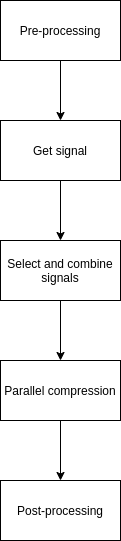
\includegraphics[width=0.3\linewidth]{figures/data_driven_surrogate_signal_extraction_methods_1_overview.png}
                
                \captionsetup{singlelinecheck=false}
                \caption{
                    A diagram showing an overview of the possible ways in which the method could be executed.
                }
                \label{fig:pca_data_driven_surrogate_signal_extraction_methods_for_dynamic_pet_methods_overview}
            \end{figure}

            Here, methods that are either simple modifications of the conventional methods, based on \gls{KRG}, or use a novel method to select and combine signals are described. These methods can be used with \gls{SAM} but for simplicity \gls{PCA} will be specifically referred to.
            
            The following subsections will address the method with respect to the diagram seen in~\Fref{fig:pca_data_driven_surrogate_signal_extraction_methods_for_dynamic_pet_methods_overview}. Additionally, a full combined diagram can be seen in~\Fref{sec:pca_data_driven_surrogate_signal_extraction_methods_for_dynamic_pet_full_overview_appendix} in~\Fref{fig:pca_data_driven_surrogate_signal_extraction_methods_for_dynamic_pet_full_overview_appendix}.

            \subsubsection{Conventional PCA} \label{sec:pca_data_driven_surrogate_signal_extraction_methods_for_dynamic_pet_methods_conventional_pca}
                \begin{figure}
                    \centering
                    
                    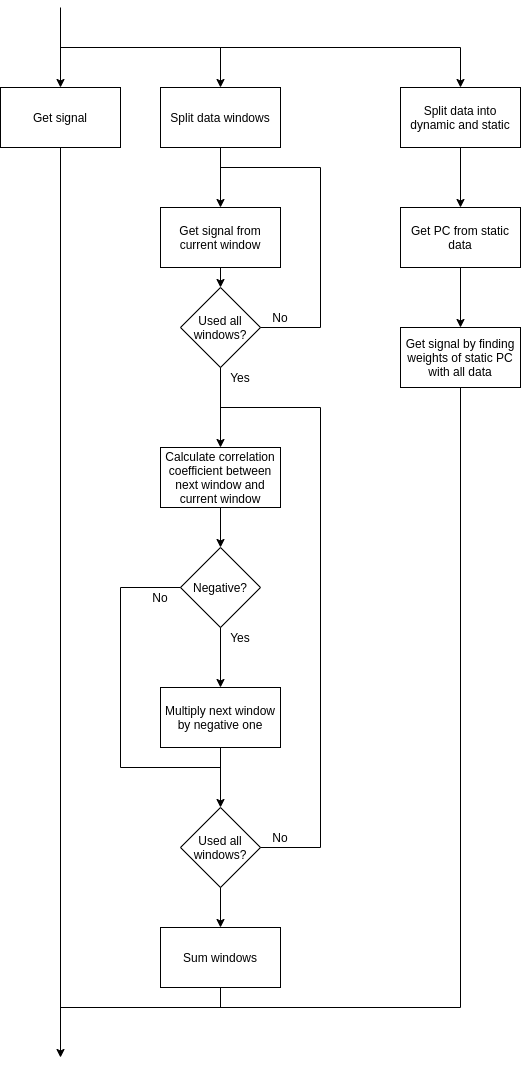
\includegraphics[width=0.7\linewidth]{figures/data_driven_surrogate_signal_extraction_methods_1_get_signal.png}
                    
                    \captionsetup{singlelinecheck=false}
                    \caption{
                        A diagram showing the methods to get a signal.
                    }
                    \label{fig:pca_data_driven_surrogate_signal_extraction_methods_for_dynamic_pet_methods_get_signal}
                \end{figure}
                
                \begin{algorithm}
                    \caption{Conventional Score}
                    \KwData{\glspl{PC}, \textit{respiratoryFrequencyWindow}}
                    \KwResult{\textit{respiratoryScore}}
                    \;
                    \textit{PSD} = \gls{FFT} on weight of current \gls{PC}\;
                    \;
                    \textit{respiratoryScore} = max value of \textit{PSD}  within \textit{respiratoryFrequencyWindow}\;
                    \;
        
                    \label{alg:pca_data_driven_surrogate_signal_extraction_methods_for_dynamic_pet_methods_conventional_pca_conventional_score_pseudo_code}
                \end{algorithm}
                
                Again, as can be seen from the diagram in~\Fref{fig:pca_data_driven_surrogate_signal_extraction_methods_for_dynamic_pet_methods_overview} there are three methods of applying \gls{PCA}. As described above in~\Fref{sec:pca_data_driven_surrogate_signal_extraction_methods_for_dynamic_pet_introduction}, \gls{PCA} is applied to the entire data set in one go as it would be if the data were from a static acquisition. The \gls{PC} containing the respiratory trace may not be the first one, generically a number of \glspl{PC} are selected and a score that maximises a signal with the appropriate respiratory features (for instance, a frequency matching the common human breathing) is selected as the \gls{SS}~\parencite{Bertolli2017}. In this implementation, to select from a number of \glspl{PC} the one which contains respiration, the signal which maximises the score seen in the pseudo code ``Conventional Score'' on page~\pageref{alg:pca_data_driven_surrogate_signal_extraction_methods_for_dynamic_pet_methods_conventional_pca_conventional_score_pseudo_code}.
                
                The generic equation for calculating the weights (or signal) from the \gls{PC} and data is
                    
                \begin{equation} \label{eq:pca_data_driven_surrogate_signal_extraction_methods_for_dynamic_pet_methods_conventional_pca_conventional_score_pseudo_code_pc_weights}
                    W = PC \cdot D
                \end{equation}
                    
                \noindent where in \Fref{eq:pca_data_driven_surrogate_signal_extraction_methods_for_dynamic_pet_methods_conventional_pca_conventional_score_pseudo_code_pc_weights} the dot denotes element-wise multiplication of the arrays, followed by summing. In fact, a similar equation is used by \gls{SAM}, where a `signed mask' is multiplied with the data and summed.

            \subsubsection{Moving Window Method} \label{sec:pca_data_driven_surrogate_signal_extraction_methods_for_dynamic_pet_methods_moving_window_method}
                \begin{figure}
                    \centering
                    
                    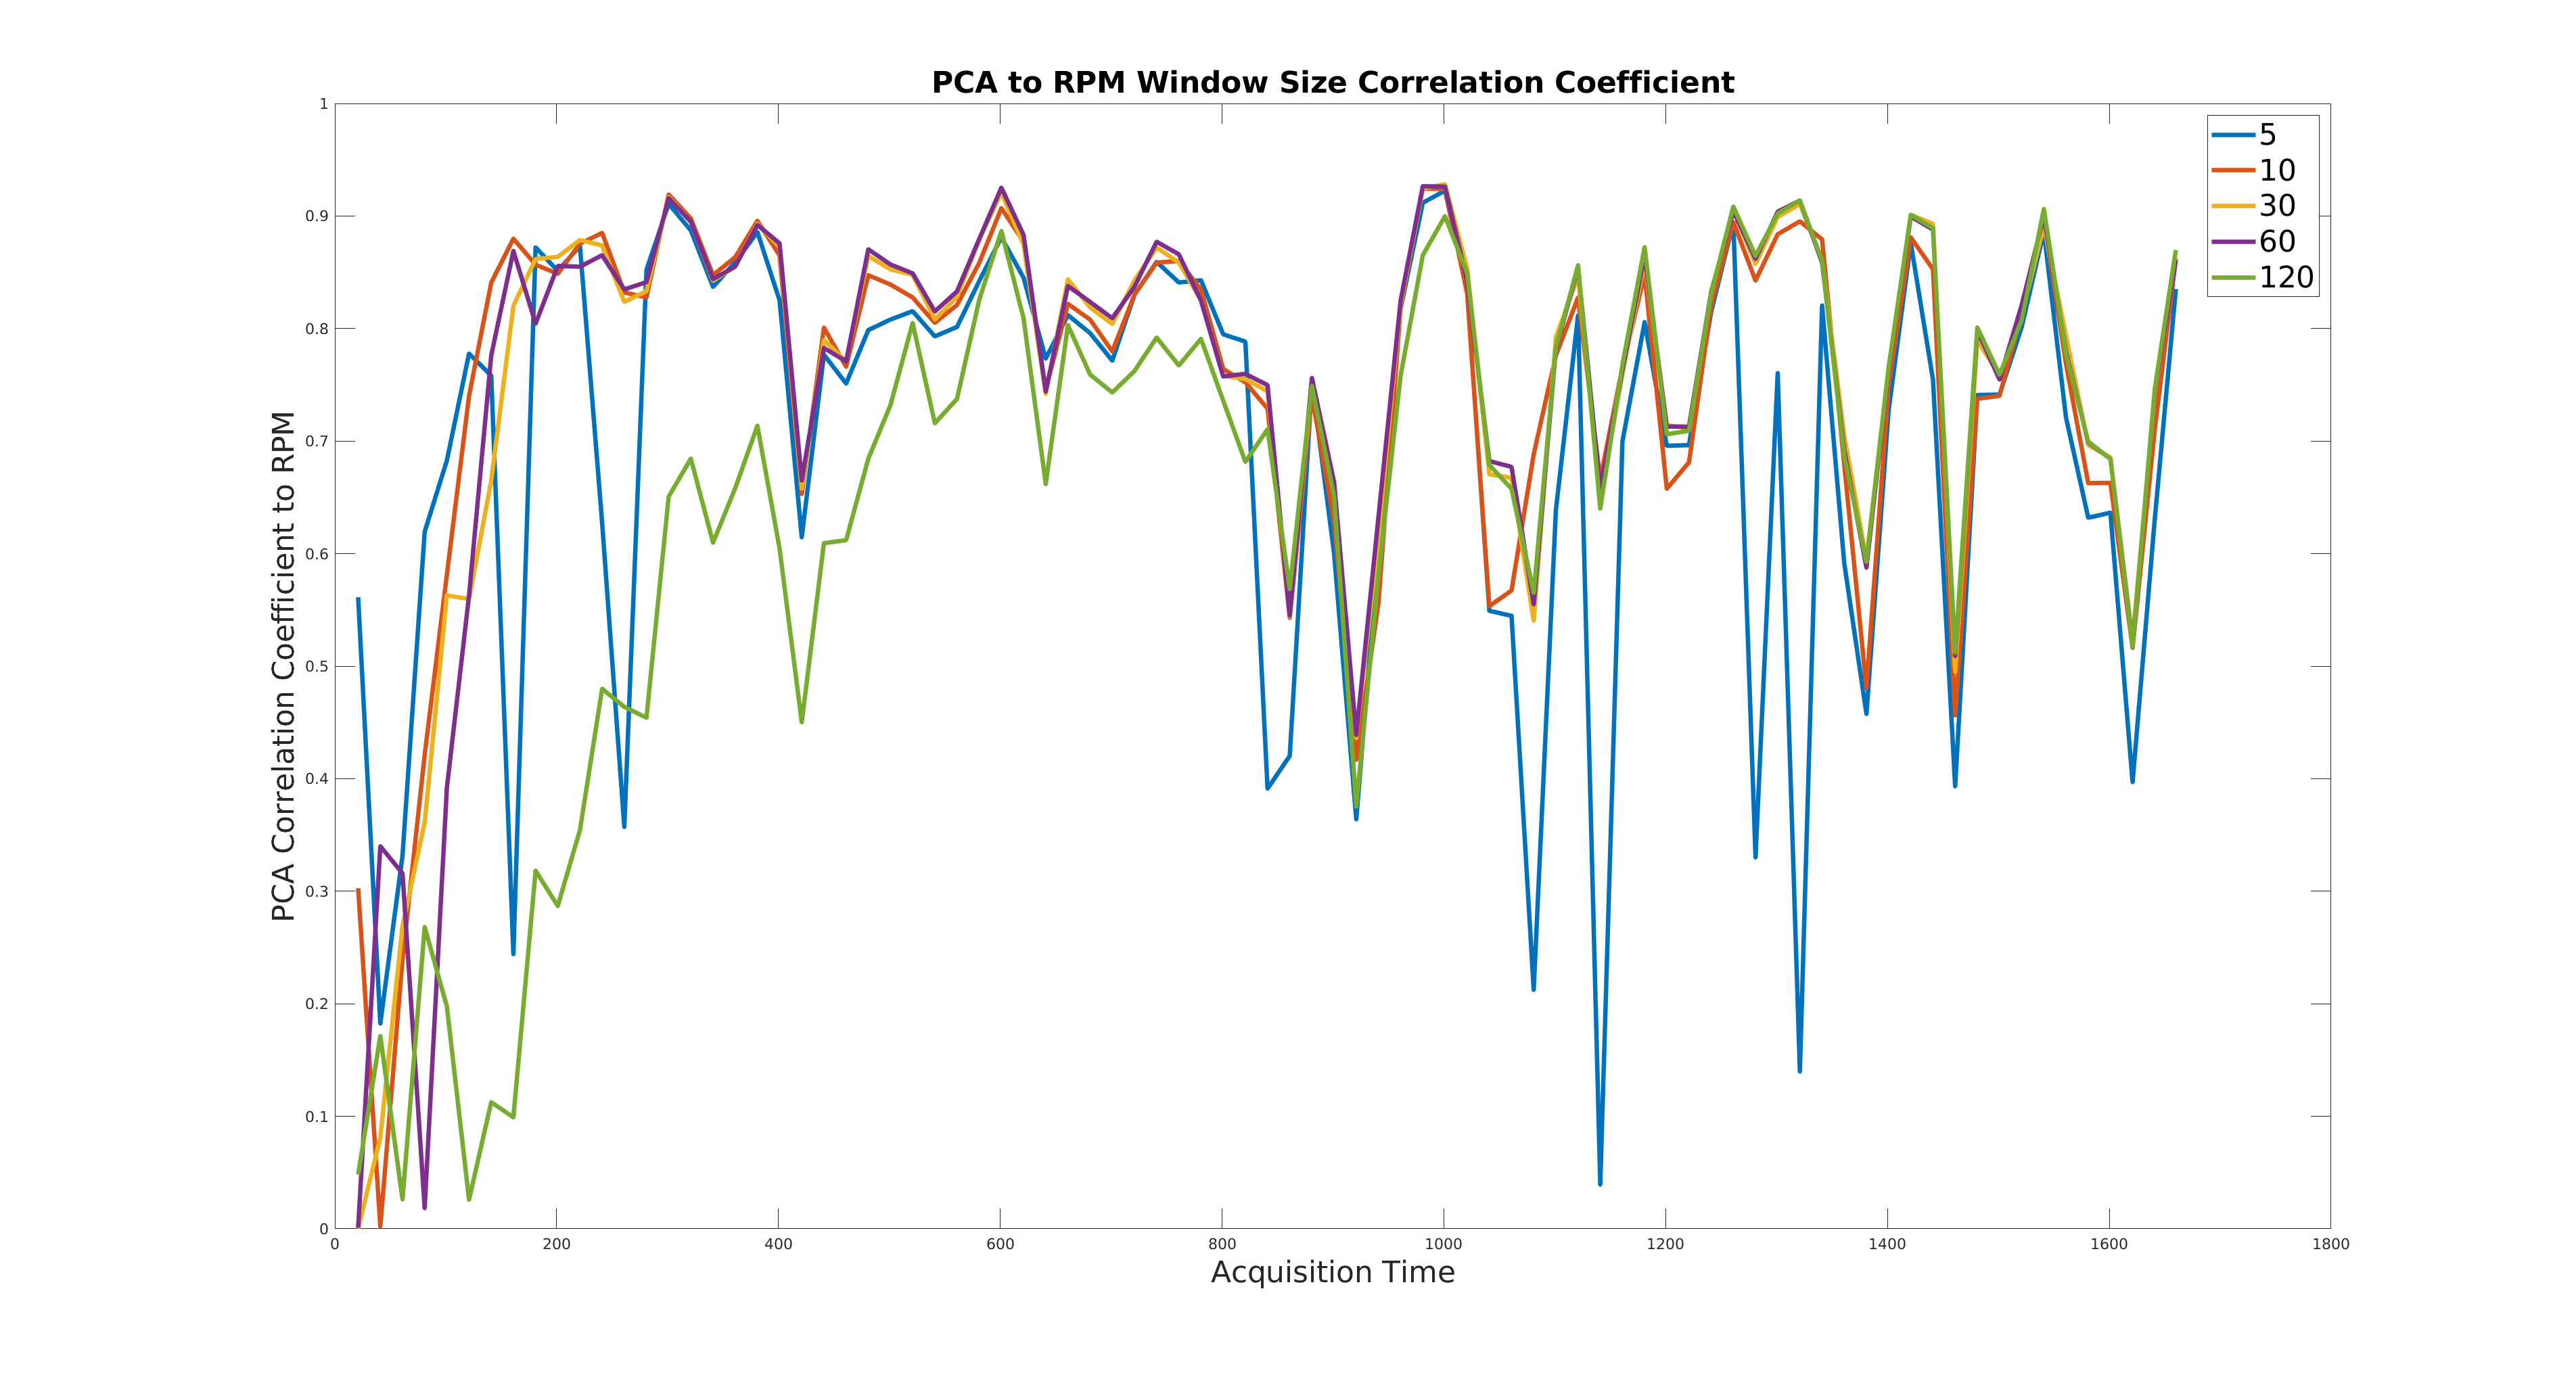
\includegraphics[width=1.0\linewidth]{figures/data_driven_surrogate_signal_extraction_methods_1_pca_window_correlation_coefficient.png}
                    
                    \captionsetup{singlelinecheck=false}
                    \caption{
                        A plot showing the moving window size optimisation for the \gls{PCA} method. For different fixed window sizes, the correlation of the extracted signal  to the \gls{RPM}  is shown for the windows sliding over the whole acquisition (taken for the first acquisition of patient one). Note that \SI{0.5}{s} time frames were used.
                    }
                    \label{fig:pca_data_driven_surrogate_signal_extraction_methods_for_dynamic_pet_methods_pca_window_correlation_coefficient}
                \end{figure}
                    
                \begin{figure}
                    \centering
                    
                    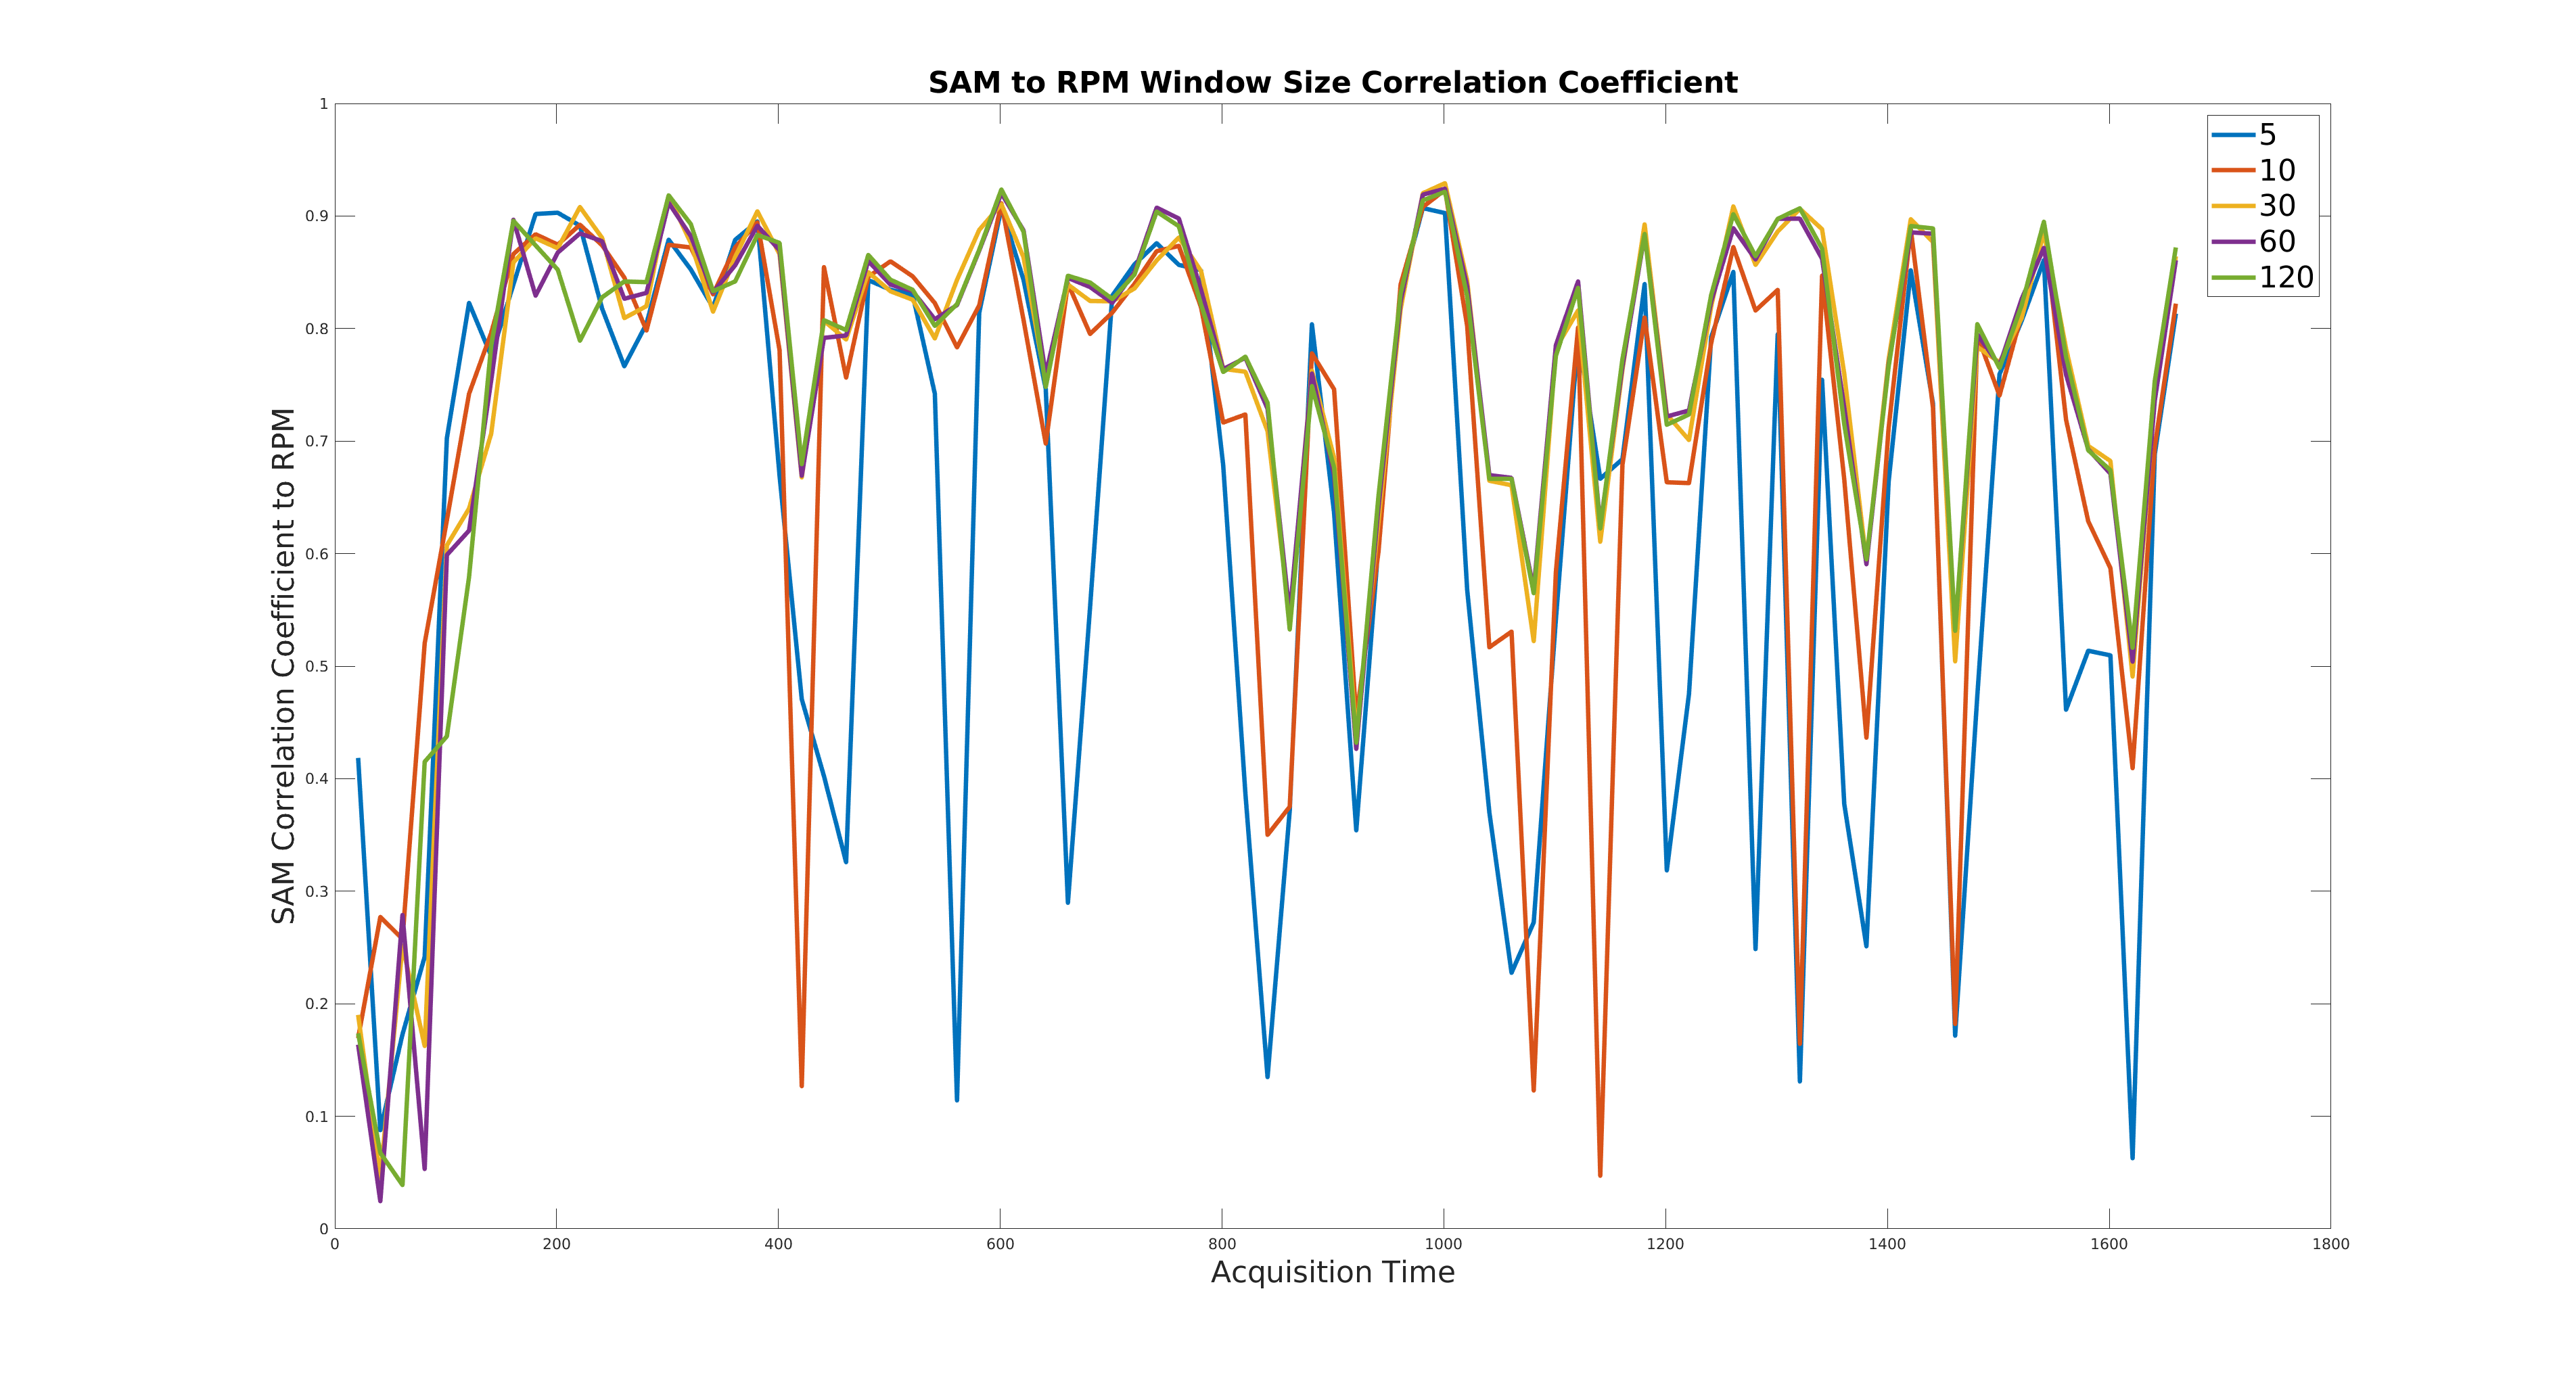
\includegraphics[width=1.0\linewidth]{figures/data_driven_surrogate_signal_extraction_methods_1_sam_window_correlation_coefficient.png}
                    
                    \captionsetup{singlelinecheck=false}
                    \caption{
                        A plot showing the moving window size optimisation for the \gls{SAM} method. For different fixed window sizes, the correlation of the extracted signal  to the \gls{RPM}  is shown for the windows sliding over the whole acquisition (taken for the first acquisition of patient one). Note that \SI{0.5}{s} time frames were used.
                    }
                    \label{fig:pca_data_driven_surrogate_signal_extraction_methods_for_dynamic_pet_methods_sam_window_correlation_coefficient}
                \end{figure}
                
                \begin{algorithm}
                    \caption{Moving Window Method}
                    \KwData{\textit{timeSeriesSinograms}, \textit{windowSizes}}
                    \KwResult{\textit{respiratorySignal}}
                    \;
                    \textit{index} = $0$\;
                    \textit{whileBool} = \textit{true}\;
                    \;
                    \While{\textit{whileBool}}{
                        \uIf{\textit{index} \textgreater length of \textit{timeSeriesSinograms}}{
                            \textit{index} = length of \textit{timeSeriesSinograms} - last \textit{windowSizes}\;
                            \;
                            \textit{whileBool} = \textit{false}\;
                        }
                        \;
                        set \textit{windowSize} to value at \textit{index} of \textit{windowSizes}\;
                        \textit{windowSignal} = fill with \textit{NaN} to \textit{index}\;
                        \textit{windowSignal} append \gls{PC} weight from \gls{PCA} for data between \textit{index} and \textit{index} + \textit{windowSize}\;
                        \textit{windowSignal} append \textit{NaN}s to length of \textit{timeSeriesSinograms}\;
                        \;
                        \textit{signals} append \textit{windowSignal}\;
                        \;
                        \textit{index} = \textit{index} + $\dfrac{\textit{windowSize}}{2}$\;
                        \;
                    }
                    \;
                    \textit{respiratorySignal} = mean of \textit{signals} ignoring \textit{NaN}\;
                    \;
                    
                    \label{alg:pca_data_driven_surrogate_signal_extraction_methods_for_dynamic_pet_methods_moving_window_pseudo_code}
                \end{algorithm}
                    
                As shown in the pseudo code ``Moving Window Method'' on page~\pageref{alg:pca_data_driven_surrogate_signal_extraction_methods_for_dynamic_pet_methods_moving_window_pseudo_code}, the data is split into a series of windows, where each subsequent window overlaps with the previous window by half its length. The motivation for attempting the Moving Window method is to increase the relative importance of motion vs kinetics. This is achieved through small windows being used at early time intervals, where the radiotracer kinetics are at their most severe, and longer windows can be used at later time intervals to reduce noise.  If \gls{SAM} is used rather than \gls{PCA},  then the method approximates \gls{KRG}~\parencite{Schleyer2014}.
                    
                The size of each window was predetermined on a small training data set. The PCA method was run with a number of fixed window sizes on a randomly selected subset of the data (specifically three patients), this data was then not used as part of any final evaluation. The window size which gave the best signal (defined as the highest correlation coefficient with the \gls{RPM} within each window) at each time interval was selected and recorded to be used with other data. Example results for this optimisation method for the moving window size can be seen in~\Fref{fig:pca_data_driven_surrogate_signal_extraction_methods_for_dynamic_pet_methods_pca_window_correlation_coefficient} and~\Fref{fig:pca_data_driven_surrogate_signal_extraction_methods_for_dynamic_pet_methods_sam_window_correlation_coefficient} for the \gls{PCA} and \gls{SAM} methods respectively.
                    
                For this method \gls{PCA} (or \gls{SAM}) is applied independently on each window and the results are averaged together, after sign correction. This is required because \glspl{PC} could produce equally valid but opposite sign results. As the sign of the signal from each window is arbitrary,  the overlapping allows for a common sign to be found by comparing the correlation coefficient of neighbouring windows and flipping windows where the correlation coefficient is negative. Other methods for sign correction are possible, for example see~\parencite{Bertolli2017, Feng2018Self-gating:PET}, as well as the sign choice in the pseudo code ``Combining \glspl{PC}'' on page~\pageref{alg:pca_data_driven_surrogate_signal_extraction_methods_for_dynamic_pet_methods_score_select_and_combine_method_combine_combine_pseudo_code}.

            \subsubsection{Late Time Interval Method} \label{sec:pca_data_driven_surrogate_signal_extraction_methods_for_dynamic_pet_methods_late_time_interval_method}
                \begin{algorithm}
                    \caption{Late Time Interval Method}
                    \KwData{\textit{timeSeriesSinograms}, \textit{lateTimeIntervalCutoff}}
                    \KwResult{\textit{respiratorySignal}}
                    \;
                    \textit{lateTimeIntervalSeriesSinograms} = split \textit{timeSeriesSinograms} from \textit{lateTimeIntervalCutoff} to end\;
                    \textit{lateTimeIntervalPC} = \gls{PC} from \gls{PCA} for \textit{lateTimeIntervalSeriesSinograms}\;
                    \textit{respiratorySignal} = \textit{lateTimeIntervalPC} $\times$ \textit{timeSeriesSinograms}\;
                    \;
        
                    \label{alg:pca_data_driven_surrogate_signal_extraction_methods_for_dynamic_pet_methods_late_time_interval_method_pseudo_code}
                \end{algorithm}
                    
                Here, a \gls{PC} from a late time interval is taken and used with all data from all time intervals with~\Fref{eq:pca_data_driven_surrogate_signal_extraction_methods_for_dynamic_pet_methods_conventional_pca_conventional_score_pseudo_code_pc_weights}. The motivation behind attempting this method was the observation that \glspl{PC} from late time interval data didn't vary significantly when different windows were selected. However, this was not true for early time interval data. It could be hypothesised, because the respiratory motion should be semi-consistent throughout the acquisition, then if a \gls{PC} is capturing the respiratory motion at late time intervals, it should do the same at early time intervals as well.
                    
                The Late Time Interval \gls{PC} method, as seen in the pseudo code ``Late Time Interval Method'' on page~\pageref{alg:pca_data_driven_surrogate_signal_extraction_methods_for_dynamic_pet_methods_late_time_interval_method_pseudo_code}, splits the data into two channels, one which only contains later time interval data, where the radiotracer kinetics have diminished, and one which contains all the data. The cutoff between early and later time interval data was determined on training data by varying the cutoff point and maximising the correlation coefficient between the output and \gls{RPM} signal for the first \SI{120}{\second} interval (between \SI{20}{\second} and \SI{140}{\second}). \gls{PCA} is applied to the later time interval data only. The \gls{PC} from the later time interval data can then be taken and multiplied by the channel containing all of the data to give the weights contributing to that \gls{PC} for all time intervals.

                A flowchart of the above can be seen in~\Fref{fig:pca_data_driven_surrogate_signal_extraction_methods_for_dynamic_pet_methods_get_signal}.

            \subsubsection{Score, Select, and Combine Method} \label{sec:pca_data_driven_surrogate_signal_extraction_methods_for_dynamic_pet_methods_score_select_and_combine_method}
                \begin{figure}
                    \centering
                    
                    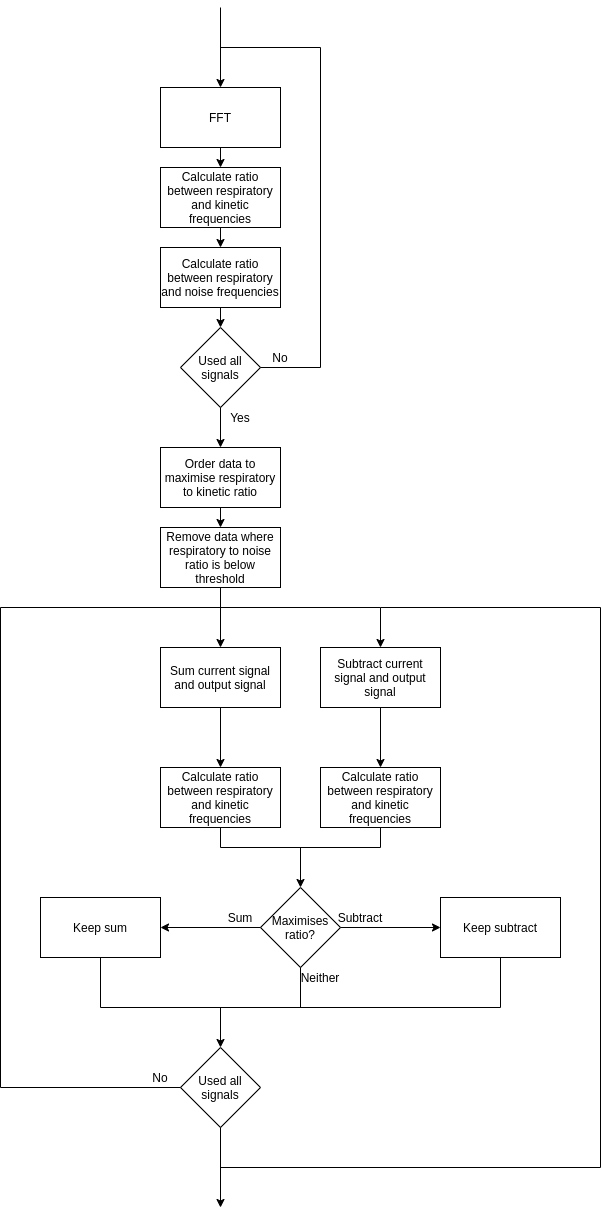
\includegraphics[width=0.7\linewidth]{figures/data_driven_surrogate_signal_extraction_methods_1_select_and_combine.png}
                    
                    \captionsetup{singlelinecheck=false}
                    \caption{
                        A diagram showing how \glspl{PC} can be selected and combined.
                    }
                    \label{fig:pca_data_driven_surrogate_signal_extraction_methods_for_dynamic_pet_methods_select_and_combine}
                \end{figure}
                
                In this section, a novel method based on a combination of previous work is described. The use of this method was inspired by the observation that signals in a frequency window of respiratory motion could be seen outside of the first few \glspl{PC}. Additionally, a significant number of these had far less of a frequency contribution in a frequency window of the radiotracer kinetics. However, the information contained in these \glspl{PC} is ignored if only one \gls{PC} is used, as in~\parencite{Thielemans2011}, and~\parencite{Bertolli2018Data-DrivenTomography}. This could lead to a reduced \gls{SNR}. The method uses a `respiratory score' and orders and combines \glspl{PC} to maximise this score. A flowchart of this can be seen in~\Fref{fig:pca_data_driven_surrogate_signal_extraction_methods_for_dynamic_pet_methods_select_and_combine}.
                    
                \paragraph{Score and Select} \label{sec:pca_data_driven_surrogate_signal_extraction_methods_for_dynamic_pet_methods_score_select_and_combine_method_score_and_select}
                    \begin{algorithm}
                        \caption{Score and Select \glspl{PC}}
                        \KwData{\glspl{PC}, \textit{scoreThreshold}}
                        \KwResult{\glspl{PC}}
                        \;
                        \For{\gls{PC} in \textit{PCs}}{
                            \textit{respiratoryScore} = get respiratory score from current \gls{PC}\;
                            \;
                            \uIf{\textit{respiratoryScore} \textgreater \textit{scoreThreshold}}{
                                \textit{respiratoryScoreList} append \textit{respiratoryScore}\;
                            }
                        }
                        \;
                        \textit{PCs} = \textit{PCs} $\times$ \textit{respiratoryScoreList}\;
                        sort \textit{PCs}\;
                        \;
        
                        \label{alg:pca_data_driven_surrogate_signal_extraction_methods_for_dynamic_pet_methods_score_select_and_combine_method_score_and_select_score_and_select_pseudo_code}
                    \end{algorithm}
        
                    \begin{algorithm}
                        \caption{Frequency Score}
                        \KwData{\glspl{PC}, \textit{kineticFrequencyWindow}, \textit{respiratoryFrequencyWindow}, \textit{noiseFrequencyWindow}}
                        \KwResult{\textit{respiratoryScore}}
                        \;
                        \textit{PSD} = \gls{FFT} on weight of current \gls{PC}\;
                        \;
                        \textit{kineticContribution} = max value of \textit{PSD} within \textit{kineticFrequencyWindow}\;
                        \textit{respiratoryContribution} = max value of \textit{PSD}  within \textit{respiratoryFrequencyWindow}\;
                        \textit{noiseContribution} = max value of \textit{PSD} within \textit{noiseFrequencyWindow}\;
                        \;
                        \textit{respiratoryKineticRatio} = $\dfrac{\textit{respiratoryContribution}}{\textit{kineticContribution}}$\;
                        \;
                        \textit{respiratoryNoiseRatio} = $\dfrac{\textit{respiratoryContribution}}{\textit{noiseContribution}}$\;
                        \;
                        \textit{respiratoryScore} = \textit{respiratoryKineticRatio} $\times$ \textit{respiratoryNoiseRatio}\;
                        \;
        
                        \label{alg:pca_data_driven_surrogate_signal_extraction_methods_for_dynamic_pet_methods_score_select_and_combine_method_score_and_select_frequency_score_pseudo_code}
                    \end{algorithm}
                
                    Several ways to calculate a score used for selecting \glspl{PC} have been developed.
                    
                    \begin{itemize}
                        \item As seen in the pseudo code ``Frequency Score'' on page~\pageref{alg:pca_data_driven_surrogate_signal_extraction_methods_for_dynamic_pet_methods_score_select_and_combine_method_score_and_select_frequency_score_pseudo_code}, \gls{PSD} analysis~\parencite{Thielemans2011} used the \gls{PSD} of the weights for each \gls{PC} to select for the \gls{PC} with the highest contribution in the respiratory window. This method is extended to account for kinetic information. In the current implementation, these \glspl{PSD} contain the frequency contribution of each signal between the frequencies of \SI{0.0}{\hertz} and \SI{1.0}{\hertz} (due to sampling the input data at \SI{1.0}{\hertz} and the Nyquist theorem~\parencite{Whittaker1915OnInterpolation-Theory, Nyquist1928CertainTheory, Shannon1949CommunicationNoise}). Frequency windows representing the content of information related to radiotracer kinetics, respiratory motion, and noise are defined. In an initial implementation they were defined as \SI{0.0}{\hertz} to \SI{0.1}{\hertz}, \SI{0.1}{\hertz} to \SI{0.4}{\hertz}, and above \SI{0.4}{\hertz} respectively~\parencite{Bertolli2017}.
                        
                        However, it was found that the choice of respiratory window boundaries was limiting, it was both too wide (so as to encourage the mislabelling of noise) and not low enough (so as to fail on slow breathers). Thus in the current implementation the respiratory window is determined by first applying the Late Time Interval \gls{PC} method and using this to estimate the frequency in this signal with the greatest magnitude. The bounds of the window were selected as being half a standard deviation from this point.
                        
                        The contribution within each window is determined for each \gls{PC} by finding the max magnitude within the windows. Ratios are then calculated between the respiratory window and the kinetic window, and the respiratory window and the noise window, and a score determined by the product of these two values.
                            
                        \item %As an extension of the above Score, Select, and Combine method in~\Fref{sec:score_method}
                        A \gls{NN} based scoring metric has also been developed to remove complexity and increase robustness when compared to the frequency scoring method~\parencite{Walker2020AutomaticAI}. %This method was originally developed by \gls{GE} to replace a similar aspect of their software suite known as the R score.            
                        The \gls{NN} is a pretrained model designed to accept a signal as input and return a score between $0.0$ and $1.0$, with a higher score indicating a more respiratory like signal. The network was trained on  scores predetermined by clinicians.
                    \end{itemize}
                    
                    Once a score for each signal has been determined the list of \glspl{PC} is sorted following this scoring as in the pseudo code ``Score and Select \glspl{PC}'' on page~\pageref{alg:pca_data_driven_surrogate_signal_extraction_methods_for_dynamic_pet_methods_score_select_and_combine_method_score_and_select_score_and_select_pseudo_code}.
                
                \paragraph{Combine} \label{sec:pca_data_driven_surrogate_signal_extraction_methods_for_dynamic_pet_methods_score_select_and_combine_method_combine}
                    \begin{algorithm}
                        \caption{Combining \glspl{PC}}
                        \KwData{\glspl{PC}}
                        \KwResult{respiratory\gls{PC}}
                        \;
                        \textit{respiratoryPC} = first \gls{PC} in \textit{PCs}\;
                        remove \textit{respiratoryPC} from \textit{PCs}\;
                        \textit{respiratoryScore} = get score from \textit{respiratoryPC}\;
                        \;
                        \For{\gls{PC} in \textit{PCs}}{
                            \textit{sumPC} = \textit{respiratoryPC} + current \gls{PC}\;
                            \textit{subtractPC} = \textit{respiratoryPC} - current \gls{PC}\;
                            \;
                            \textit{sumRespiratoryScore} = get respiratory score from \textit{sumPC}\;
                            \textit{subtractRespiratoryScore} = get respiratory score from \textit{subtractPC}\;
                            \;
                            \eIf{\textit{sumRespiratoryScore} \textgreater \textit{respiratoryScore}}{
                                \textit{respiratoryPC} = \textit{sumPC}\;
                                \textit{respiratoryScore} = \textit{sumRespiratoryScore}\;
                            }{
                                \uIf{\textit{subtractRespiratoryScore} \textgreater \textit{respiratoryScore}}{
                                    \textit{respiratoryPC} = \textit{subtractPC}\;
                                    \textit{respiratoryScore} = \textit{subtractRespiratoryScore}\;
                                }
                            }
                        }
                        \;
        
                        \label{alg:pca_data_driven_surrogate_signal_extraction_methods_for_dynamic_pet_methods_score_select_and_combine_method_combine_combine_pseudo_code}
                    \end{algorithm}
                    
                    After the \glspl{PC} are sorted from high to low score they are then iterated over, both being summed and subtracted (with a weighting, the score) and a new score is found for both resulting signals. If one of the signals increases this score then it becomes the new best \gls{PC} and goes forward to the next iteration. \glspl{PC} are both summed and subtracted to handle the arbitrary sign problem mentioned earlier in~\Fref{sec:pca_data_driven_surrogate_signal_extraction_methods_for_dynamic_pet_methods_moving_window_method}~\parencite{Bertolli2017}. The arbitrary sign flip problem is less pronounced for \gls{NN} scoring. This is due to a bias towards signals in a certain orientation, because clinicians have a tendency to score \glspl{SS} in a particular orientation higher.
                    
                    A similar method of combining signals can be seen in~\parencite{Kesner2010AMethods}. However, the method presented here has the advantage over the method presented in~\parencite{Kesner2010AMethods}. The metric to define a good signal specifically looks to maximise a value related to the behaviour desired, while in~\parencite{Kesner2010AMethods}, the standard deviation is maximised. In addition, the proposed method computes the metric based on signals derived from \glspl{PC} as opposed to single voxel or sinogram bin values, which should lead to noise reduction.
                    
                    Please note that the pseudo code ``Combining \glspl{PC}'' on page~\pageref{alg:pca_data_driven_surrogate_signal_extraction_methods_for_dynamic_pet_methods_score_select_and_combine_method_combine_combine_pseudo_code} is described in terms of \glspl{PC}. In fact, a simpler version just sums and subtracts the corresponding signals, this will give the same final signal. 
                
                    In the current implementation, this method is applied on all time intervals at once. It is possible to integrate this method with the Late Time Interval method in~\Fref{sec:pca_data_driven_surrogate_signal_extraction_methods_for_dynamic_pet_methods_late_time_interval_method} or the Moving Window method. However, this has not been demonstrated here.
                    
        \subsection{Evaluation} \label{sec:pca_data_driven_surrogate_signal_extraction_methods_for_dynamic_pet_evaluation}
            Here, it is discussed where data was acquired from and then how this was prepared for evaluation. A suite of methods which can be applied generally to \glspl{SS} (both from dynamic as well as potentially static acquisitions) in order to combat issues such as noise and outliers is also presented. Finally, in this section, the methods highlighted in~\Fref{sec:pca_data_driven_surrogate_signal_extraction_methods_for_dynamic_pet_methods} are shown how they will be evaluated in~\Fref{sec:pca_data_driven_surrogate_signal_extraction_methods_for_dynamic_pet_results}

            \subsubsection{Data Acquisition} \label{sec:pca_data_driven_surrogate_signal_extraction_methods_for_dynamic_pet_evaluation_data_acquisition}
                Data used was acquired from a research study with patients suffering from \gls{IPF}~\parencite{Emond2020EffectReconstruction}. $21$ dynamic \gls{18F-FDG} acquisitions, with a \gls{FOV} covering the upper lung and heart, were acquired on a \gls{GE} Discovery $710$ in list-mode. Data used in this study was from the first \SI{20}{\minute} with the acquisition starting roughly \SI{20}{\second} before injection of the radiotracer. An external surrogate signal was acquired in parallel using an \gls{RPM}~\parencite{Oh2019OptimalTreatment}.

            \subsubsection{Data Preparation} \label{sec:pca_data_driven_surrogate_signal_extraction_methods_for_dynamic_pet_evaluation_data_preparation}
                \begin{figure}
                    \centering
                    
                    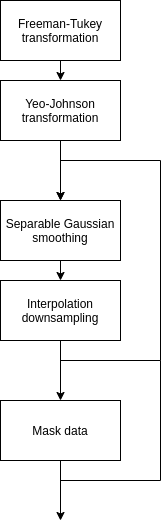
\includegraphics[width=0.4\linewidth]{figures/data_driven_surrogate_signal_extraction_methods_1_pre_processing.png}
                    
                    \captionsetup{singlelinecheck=false}
                    \caption{
                        A diagram showing pre-processing performed.
                    }
                    \label{fig:pca_data_driven_surrogate_signal_extraction_methods_for_dynamic_pet_evaluation_data_preparation_pre_processing}
                \end{figure}
                
                \gls{TOF} data were unlisted into low spatial resolution sinograms, each with a time frame duration of \SI{500}{\milli\second}, using the \gls{GE} PetToolbox, following~\parencite{Bertolli2017DataData}, resulting in sinograms with dimensions $95\times16\times47\times11$ (radial positions$\times$angles$\times$transaxial plane$\times$\gls{TOF}). To extract respiratory variation, the sampling rate of the \gls{PET} sinograms was chosen as \SI{2}{\hertz}, so as to attempt to mitigate the effect of cardiac motion~\parencite{Bertolli2018Data-DrivenTomography}.
                
                Data was pre-processed element-wise by first applying a Freeman-Tukey transformation~\parencite{Freeman1950TransformationsRoot} before then applying a Yeo-Johnson power transformation~\parencite{Yeo2000ASymmetry}, to transform the Poisson distributed data to be more Gaussian-like. The Yeo-Johnson power transformation was added as it was found that this gave more robust results.
                
                The Freeman-Tukey transformation is defined as
                
                \begin{equation} \label{eq:pca_data_driven_surrogate_signal_extraction_methods_for_dynamic_pet_evaluation_data_preparation_freeman_tukey}
                    X_g = \sqrt{X_p + 1} + \sqrt{X_p}
                \end{equation}
                
                \noindent where in~\Fref{eq:pca_data_driven_surrogate_signal_extraction_methods_for_dynamic_pet_evaluation_data_preparation_freeman_tukey} $X_g$ is the resultant, approximately Gaussian distributed, variable and $X_p$ is the original Poisson distributed variable $S_p$~\parencite{Freeman1950TransformationsRoot}.
                
                The Yeo-Johnson power transformation is defined as
                
                \begin{equation} \label{eq:pca_data_driven_surrogate_signal_extraction_methods_for_dynamic_pet_evaluation_data_preparation_yeo_johnson}
                    X_g =   \begin{cases}
                                ((X + 1)^\lambda - 1) / \lambda                     & \quad \text{if } \lambda \neq 0 \text{, } X \geq 0 \\
                                \log(X + 1)                                         & \quad \text{if } \lambda = 0 \text{, } X \geq 0    \\
                                -[(-X + 1)^{(2 - \lambda)} - 1)] / (2 - \lambda)    & \quad \text{if } \lambda \neq 2 \text{, } X < 0    \\
                                -\log(-X + 1)                                       & \quad \text{if } \lambda = 2 \text{, } X < 0
                            \end{cases}
                \end{equation}
                
                \noindent where in~\Fref{eq:pca_data_driven_surrogate_signal_extraction_methods_for_dynamic_pet_evaluation_data_preparation_yeo_johnson} again $X_g$ is the resultant, approximately Gaussian distributed, variable and $X$ is the original distributed variable $S_p$. The $\lambda$ parameter is determined by minimising the \gls{KLD} between normal distributions and the transformed distribution~\parencite{Yeo2000ASymmetry}. 
                
                In the current implementation, these transformations are applied element-wise on the (Poisson distributed) TOF sinogram $S_p$, but with a single $\lambda$ determined from all of the data, although it would be feasible to find different $\lambda$ values for every element in the sinogram, resulting in
                
                \begin{equation} \label{eq:pca_data_driven_surrogate_signal_extraction_methods_for_dynamic_pet_evaluation_data_preparation_freeman_tukey_yeo_johnson}
                    S_g = \mathrm{YJ}(\mathrm{FT}(S_p))
                \end{equation}
                
                \noindent where in~\Fref{eq:pca_data_driven_surrogate_signal_extraction_methods_for_dynamic_pet_evaluation_data_preparation_freeman_tukey_yeo_johnson} $FT$ is the Freeman-Tukey transformation, as in~\Fref{eq:pca_data_driven_surrogate_signal_extraction_methods_for_dynamic_pet_evaluation_data_preparation_freeman_tukey}, and $YJ$ is Yeo-Johnson power transformation, as in~\Fref{eq:pca_data_driven_surrogate_signal_extraction_methods_for_dynamic_pet_evaluation_data_preparation_yeo_johnson}.
                
                It has been found through experimentation that Gaussian smoothing of the resulting sinograms can improve results, especially in the case of the \gls{SAM} methods~\parencite{Thielemans2013ComparisonData}. Further downsampling was performed post-smoothing to reduce memory usage. Linear interpolation was used as it was shown in a preliminary investigation to give  satisfactory results at little computational cost.
                
                Finally, it has been found that the introduction of a mask to further aid in the reduction of noise is beneficial~\parencite{Thielemans2011}. The mask itself is defined as being true for any value, in the sinogram, above a predetermined threshold. Values not in the mask are removed prior to further execution, this is because these values can be assumed to mostly be noise. Note that a mask can also be used to eliminate parts of the data potentially affected by non-respiratory movement~\parencite{Bertolli2018Data-DrivenTomography}, but this has not been implemented in the current work.
        
                Values for the Gaussian smoothing, spatial downsampling, and the threshold of the mask were determined using a grid search on a randomly selected subset of the data (specifically three patients), this data was then not used as part of any final evaluation.

                A flowchart of the above can be seen in~\Fref{fig:pca_data_driven_surrogate_signal_extraction_methods_for_dynamic_pet_evaluation_data_preparation_pre_processing}.
            
            \subsubsection{Post-Processing} \label{sec:pca_data_driven_surrogate_signal_extraction_methods_for_dynamic_pet_evaluation_post_processing}
                \begin{figure}
                    \centering
                    
                    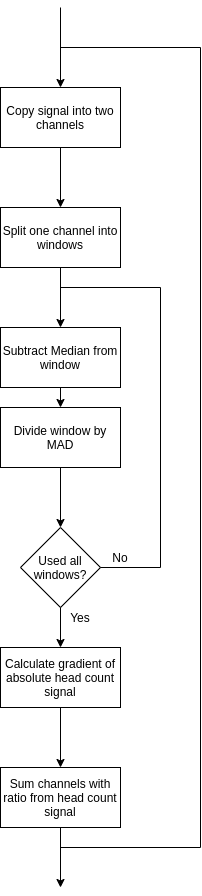
\includegraphics[width=0.3\linewidth]{figures/data_driven_surrogate_signal_extraction_methods_1_parallel_compression.png}
                    
                    \captionsetup{singlelinecheck=false}
                    \caption{
                        A diagram showing the parallel compression method.
                    }
                    \label{fig:pca_data_driven_surrogate_signal_extraction_methods_for_dynamic_pet_evaluation_post_processing_parallel_compression}
                \end{figure}
                
                \begin{figure}
                    \centering
                    
                    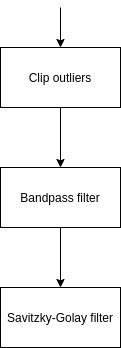
\includegraphics[width=0.5\linewidth]{figures/data_driven_surrogate_signal_extraction_methods_1_post_processing.png}
                    
                    \captionsetup{singlelinecheck=false}
                    \caption{
                        A diagram showing the post-processing performed.
                    }
                    \label{fig:pca_data_driven_surrogate_signal_extraction_methods_for_dynamic_pet_evaluation_post_processing_post_processing}
                \end{figure}
                
                A flowchart of the method can be seen in~\Fref{fig:pca_data_driven_surrogate_signal_extraction_methods_for_dynamic_pet_evaluation_post_processing_parallel_compression} and~\Fref{fig:pca_data_driven_surrogate_signal_extraction_methods_for_dynamic_pet_evaluation_post_processing_post_processing}.
                
                Regardless of the method used there are still some effects of the radiotracer kinetics to be expected at early time intervals and noise throughout. Thus a method is proposed here to aid with the remaining radiotracer kinetics and smoothing to help with noise in the extracted \gls{SS}. The same post-processing is used regardless of the method to extract the \gls{SS}.
                    
                \begin{itemize}
                    \item Firstly there is, what shall be referred to as ``parallel compression''. This is a method borrowed from audio engineering (appearing notably in Dolby A noise reduction). The signal is split into two channels, one has its dynamic range reduced (through a process such as compression) while the other passes unchanged before they are summed back together~\parencite{Izhaki2012MixingTools}. This has the effect of reducing large differences in the dynamic range of the signal without losing a lot of breath to breath variability. In order to achieve this here, the signal is split into two channels (in this case this means replicating the signal such that there are two copies) and one of those channels is further split into a series of small moving windows. Each window is then normalised, this channel has its windows averaged back together before being combined with the unadulterated channel. The channels are combined following the gradient of the head count (the head count signal being defined as the sum of counts in each sinogram over time). The absolute value of the signal is first taken before it is normalised between zero and one. Then the low dynamic range and high dynamic range signals are summed using the magnitude of the processed head count signal as a weighting. At time intervals where the magnitude of the processed head count signal is greater, more of the compressed/normalised signal is summed compared to the non-compressed/non-normalised signal. The total weighting is always equal to one, to maintain the scale of the signal.
                        
                    \item Even though most of the large macro changes in intensity are remedied by parallel compression, some momentary spikes are still apparent. Thus, outliers are removed where they are outside a threshold of the quartile of the signal and new values are interpolated.
                        
                    \item Finally, smoothing is applied through the use of a bandpass filter (specifically a pseudo-sinc filter) followed by a Savitzky-Golay filter~\parencite{Savitzky1964SmoothingProcedures}.
                \end{itemize}

            \subsubsection{Evaluation Methods} \label{sec:pca_data_driven_surrogate_signal_extraction_methods_for_dynamic_pet_evaluation_evaluation_methods}
                For evaluation of the results the correlation coefficient of each surrogate signal between each method and the \gls{RPM}, for all acquisitions, has been calculated. The correlation coefficient has been calculated for both the first \SI{120}{\second} (ignoring the first \SI{20}{\second}) and also the entire acquisition (between \SI{20}{\second} and \SI{1200}{\second}).
                
                All methods were evaluated with \gls{PCA}. Results for the Moving Window \gls{SAM} method were also included as this approximates \gls{KRG}.
                While the Conventional and Late Time Interval methods can also be implemented using \gls{SAM}, corresponding results are not shown here.
        
                Parameters for the methods have been selected using a grid search on a randomly selected subset of the data (specifically three patients), this data was then not used as part of any final evaluation. The parameters were optimised by maximising the correlation coefficient between the surrogate signal and the \gls{RPM} for the first \SI{120}{\second} of usable data (between \SI{20}{\second} and \SI{140}{\second}) due to there being initially no counts in the \gls{FOV}.

        \subsection{Results} \label{sec:pca_data_driven_surrogate_signal_extraction_methods_for_dynamic_pet_results}
            \begin{figure}
                \centering
                
                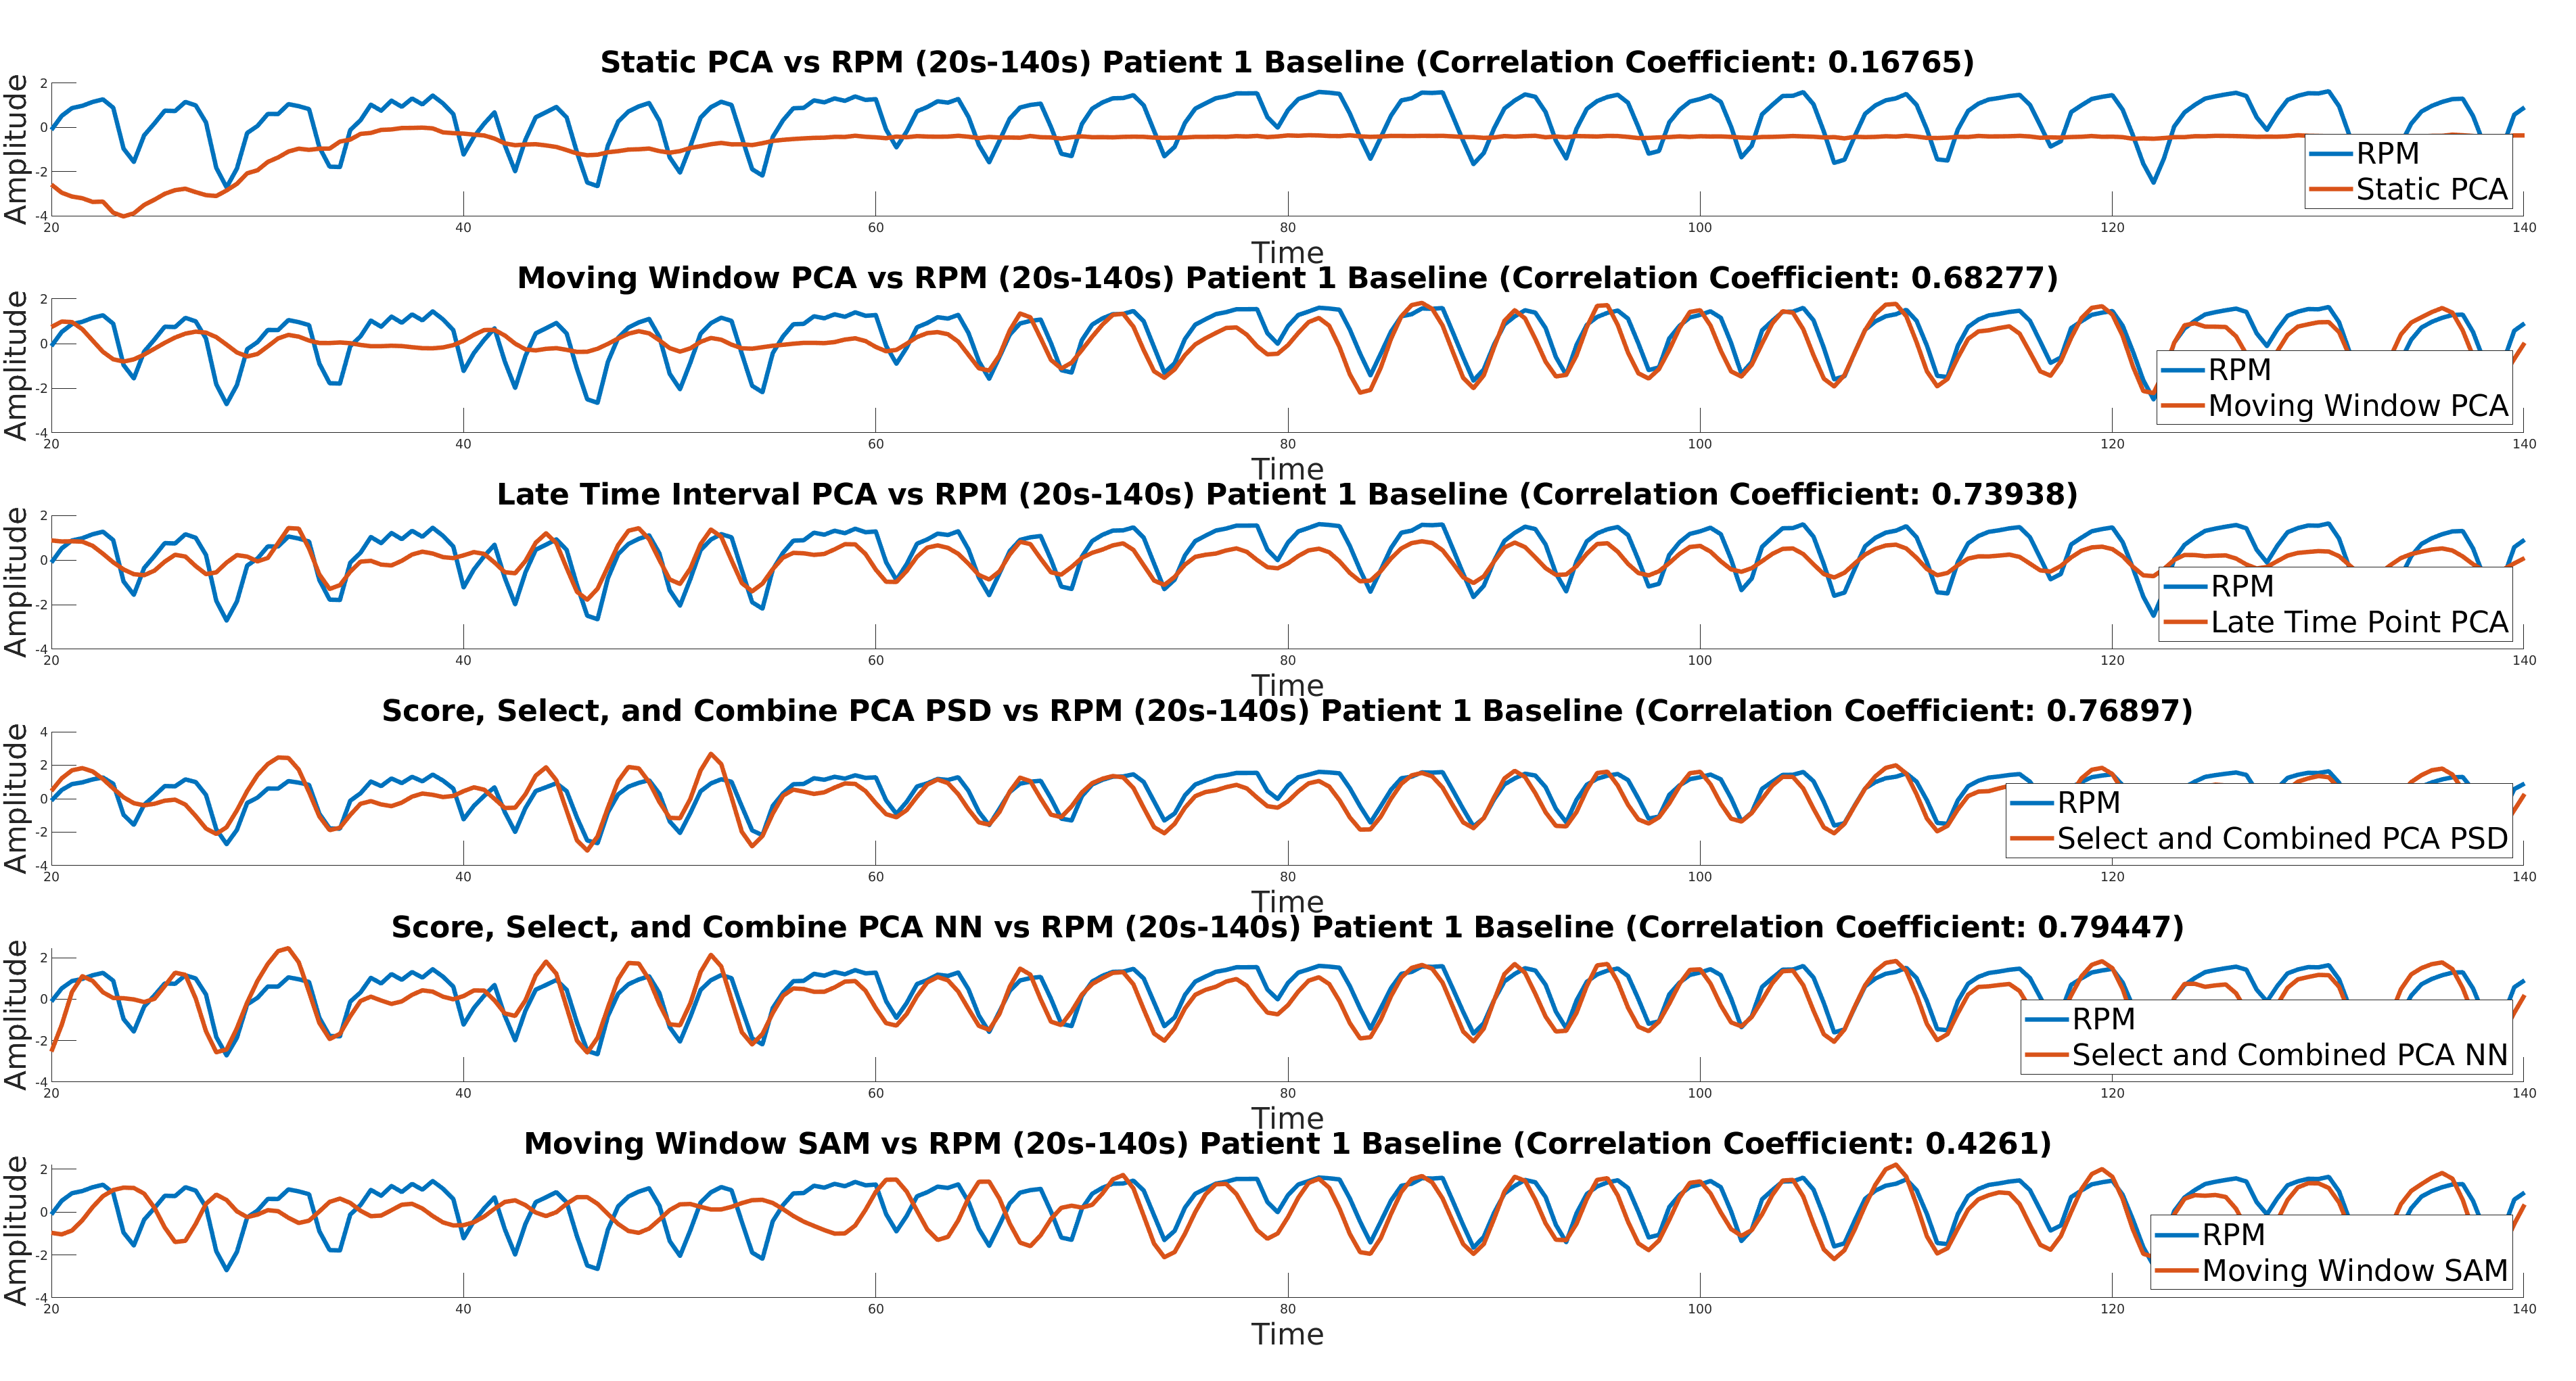
\includegraphics[width=1.0\linewidth]{figures/data_driven_surrogate_signal_extraction_methods_1_patient_one_output.png}
                
                \captionsetup{singlelinecheck=false}
                \caption{
                    Output of each method compared to the \gls{RPM} for the first usable \SI{120}{\second} (between \SI{20}{\second} and \SI{140}{\second}) (taken for the first acquisition of patient one). This is for Conventional \gls{PCA}, Moving Window \gls{PCA}, Late Time Interval \gls{PC}, Score, Select, and Combine using frequency and \gls{NN} scoring, and the Moving Window \gls{SAM} method.
                }
                \label{fig:patient_one_output}
            \end{figure}
            
            \begin{figure}
                \centering
                
                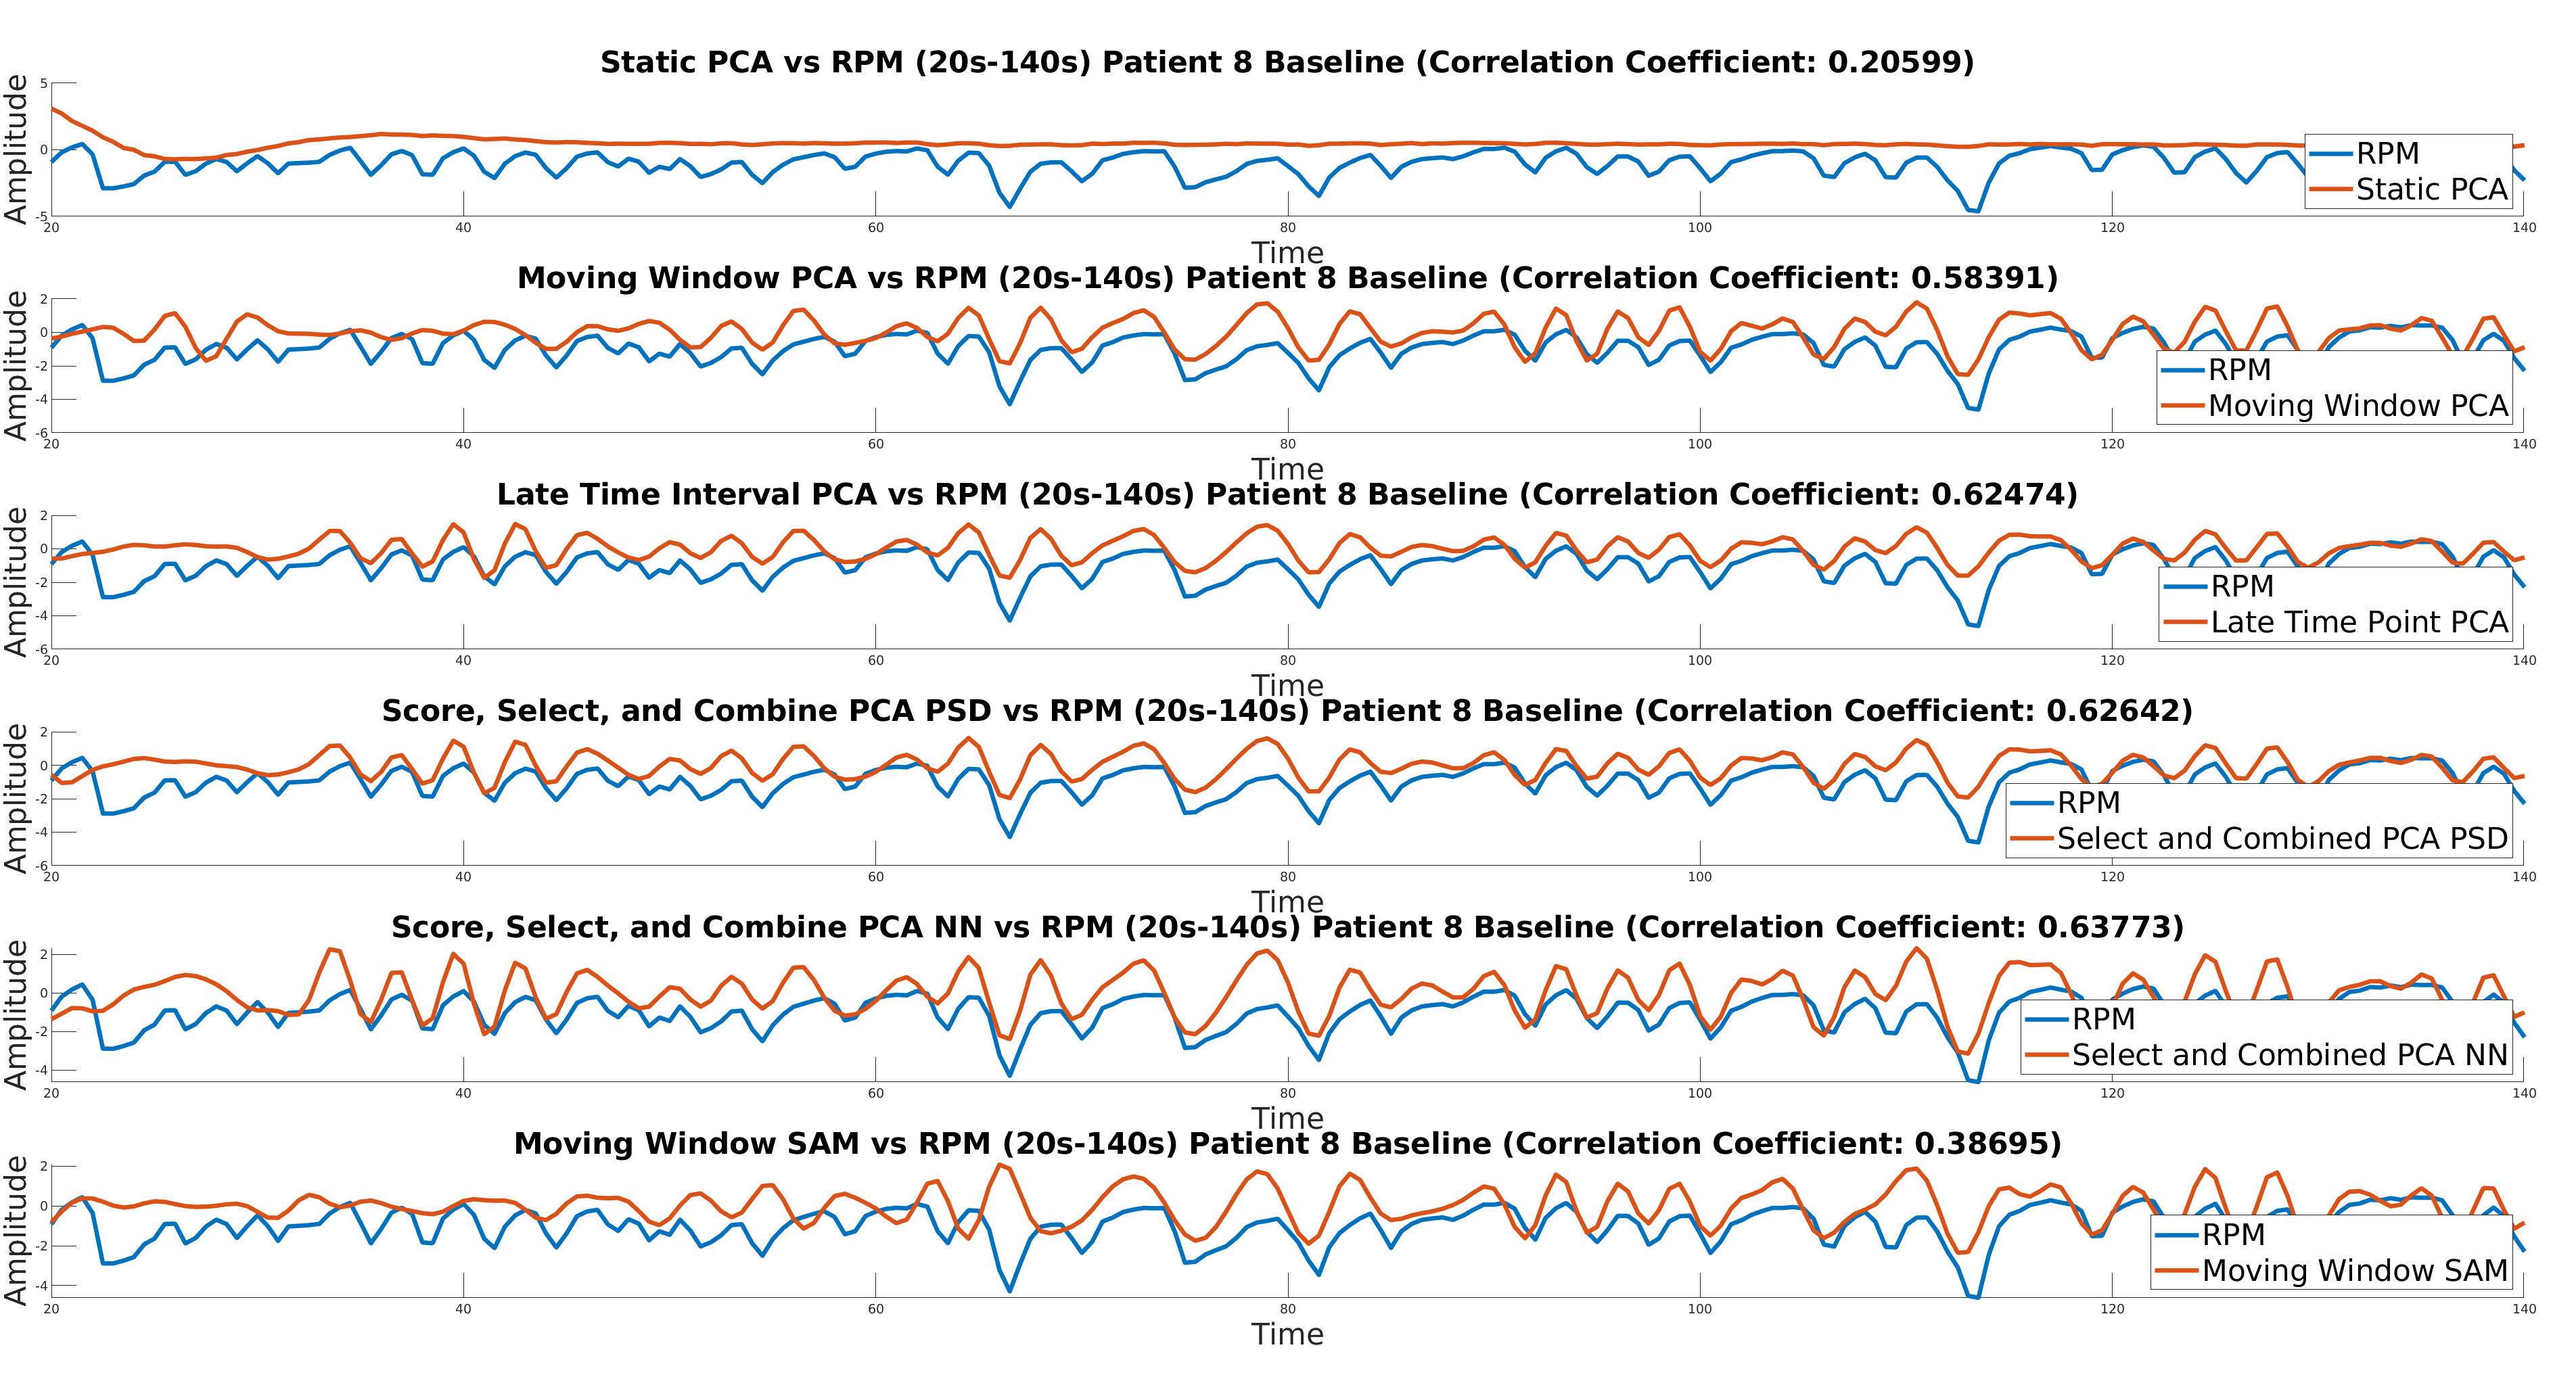
\includegraphics[width=1.0\linewidth]{figures/data_driven_surrogate_signal_extraction_methods_1_patient_eight_output.png}
                
                \captionsetup{singlelinecheck=false}
                \caption{
                    Output of each method compared to the \gls{RPM} for the first usable \SI{120}{\second} (between \SI{20}{\second} and \SI{140}{\second}) (taken for the first acquisition of patient eight). This is for Conventional \gls{PCA}, Moving Window \gls{PCA}, Late Time Interval \gls{PC}, Score, Select, and Combine using frequency and \gls{NN} scoring, and the Moving Window \gls{SAM} method.
                }
                \label{fig:patient_eight_output}
            \end{figure}
        
            \begin{figure}
                \centering
                
                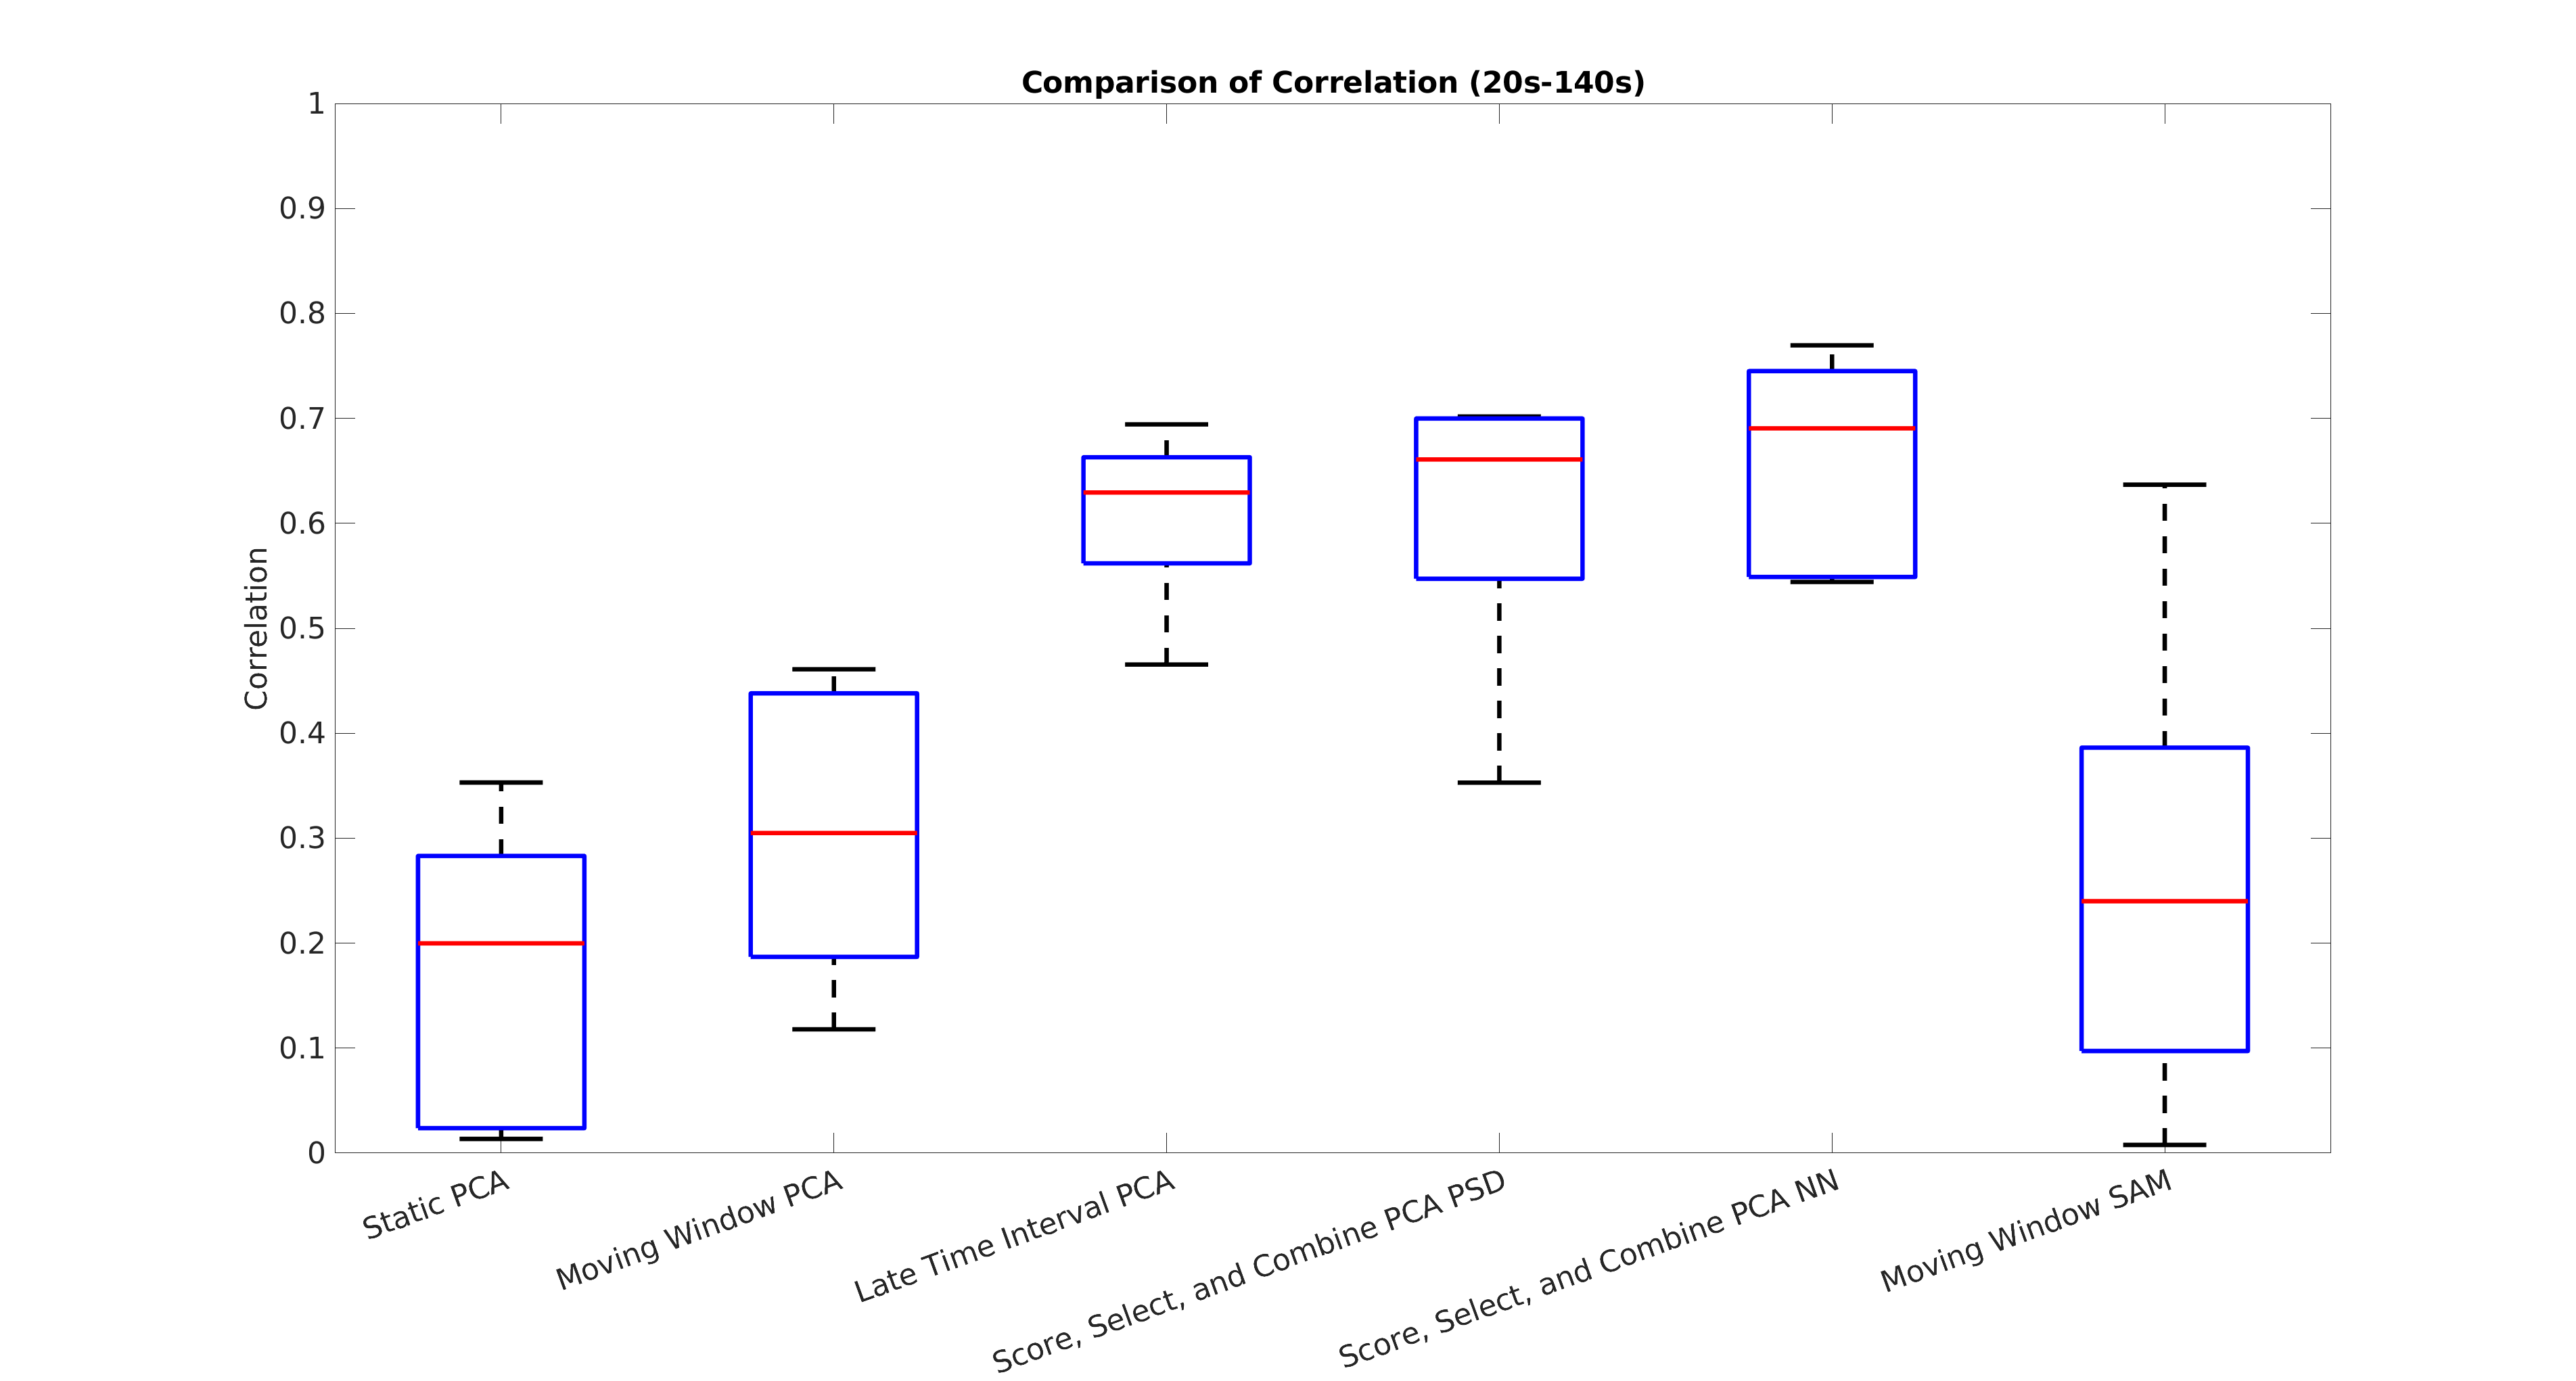
\includegraphics[width=1.0\linewidth]{figures/data_driven_surrogate_signal_extraction_methods_1_box_plot_early.png}
                
                \captionsetup{singlelinecheck=false}
                \caption{
                    A box plot showing for each method its correlation coefficient to the \gls{RPM} for the first usable \SI{120}{\second} (between \SI{20}{\second} and \SI{140}{\second}) (taken for seven acquisitions). This is for Conventional \gls{PCA}, Moving Window \gls{PCA}, Late Time Interval \gls{PC}, Score, Select, and Combine using frequency and \gls{NN} scoring, and the Moving Window \gls{SAM} method.
                }
                \label{fig:box_plot_early}
            \end{figure}
        
            \begin{figure}
                \centering
                
                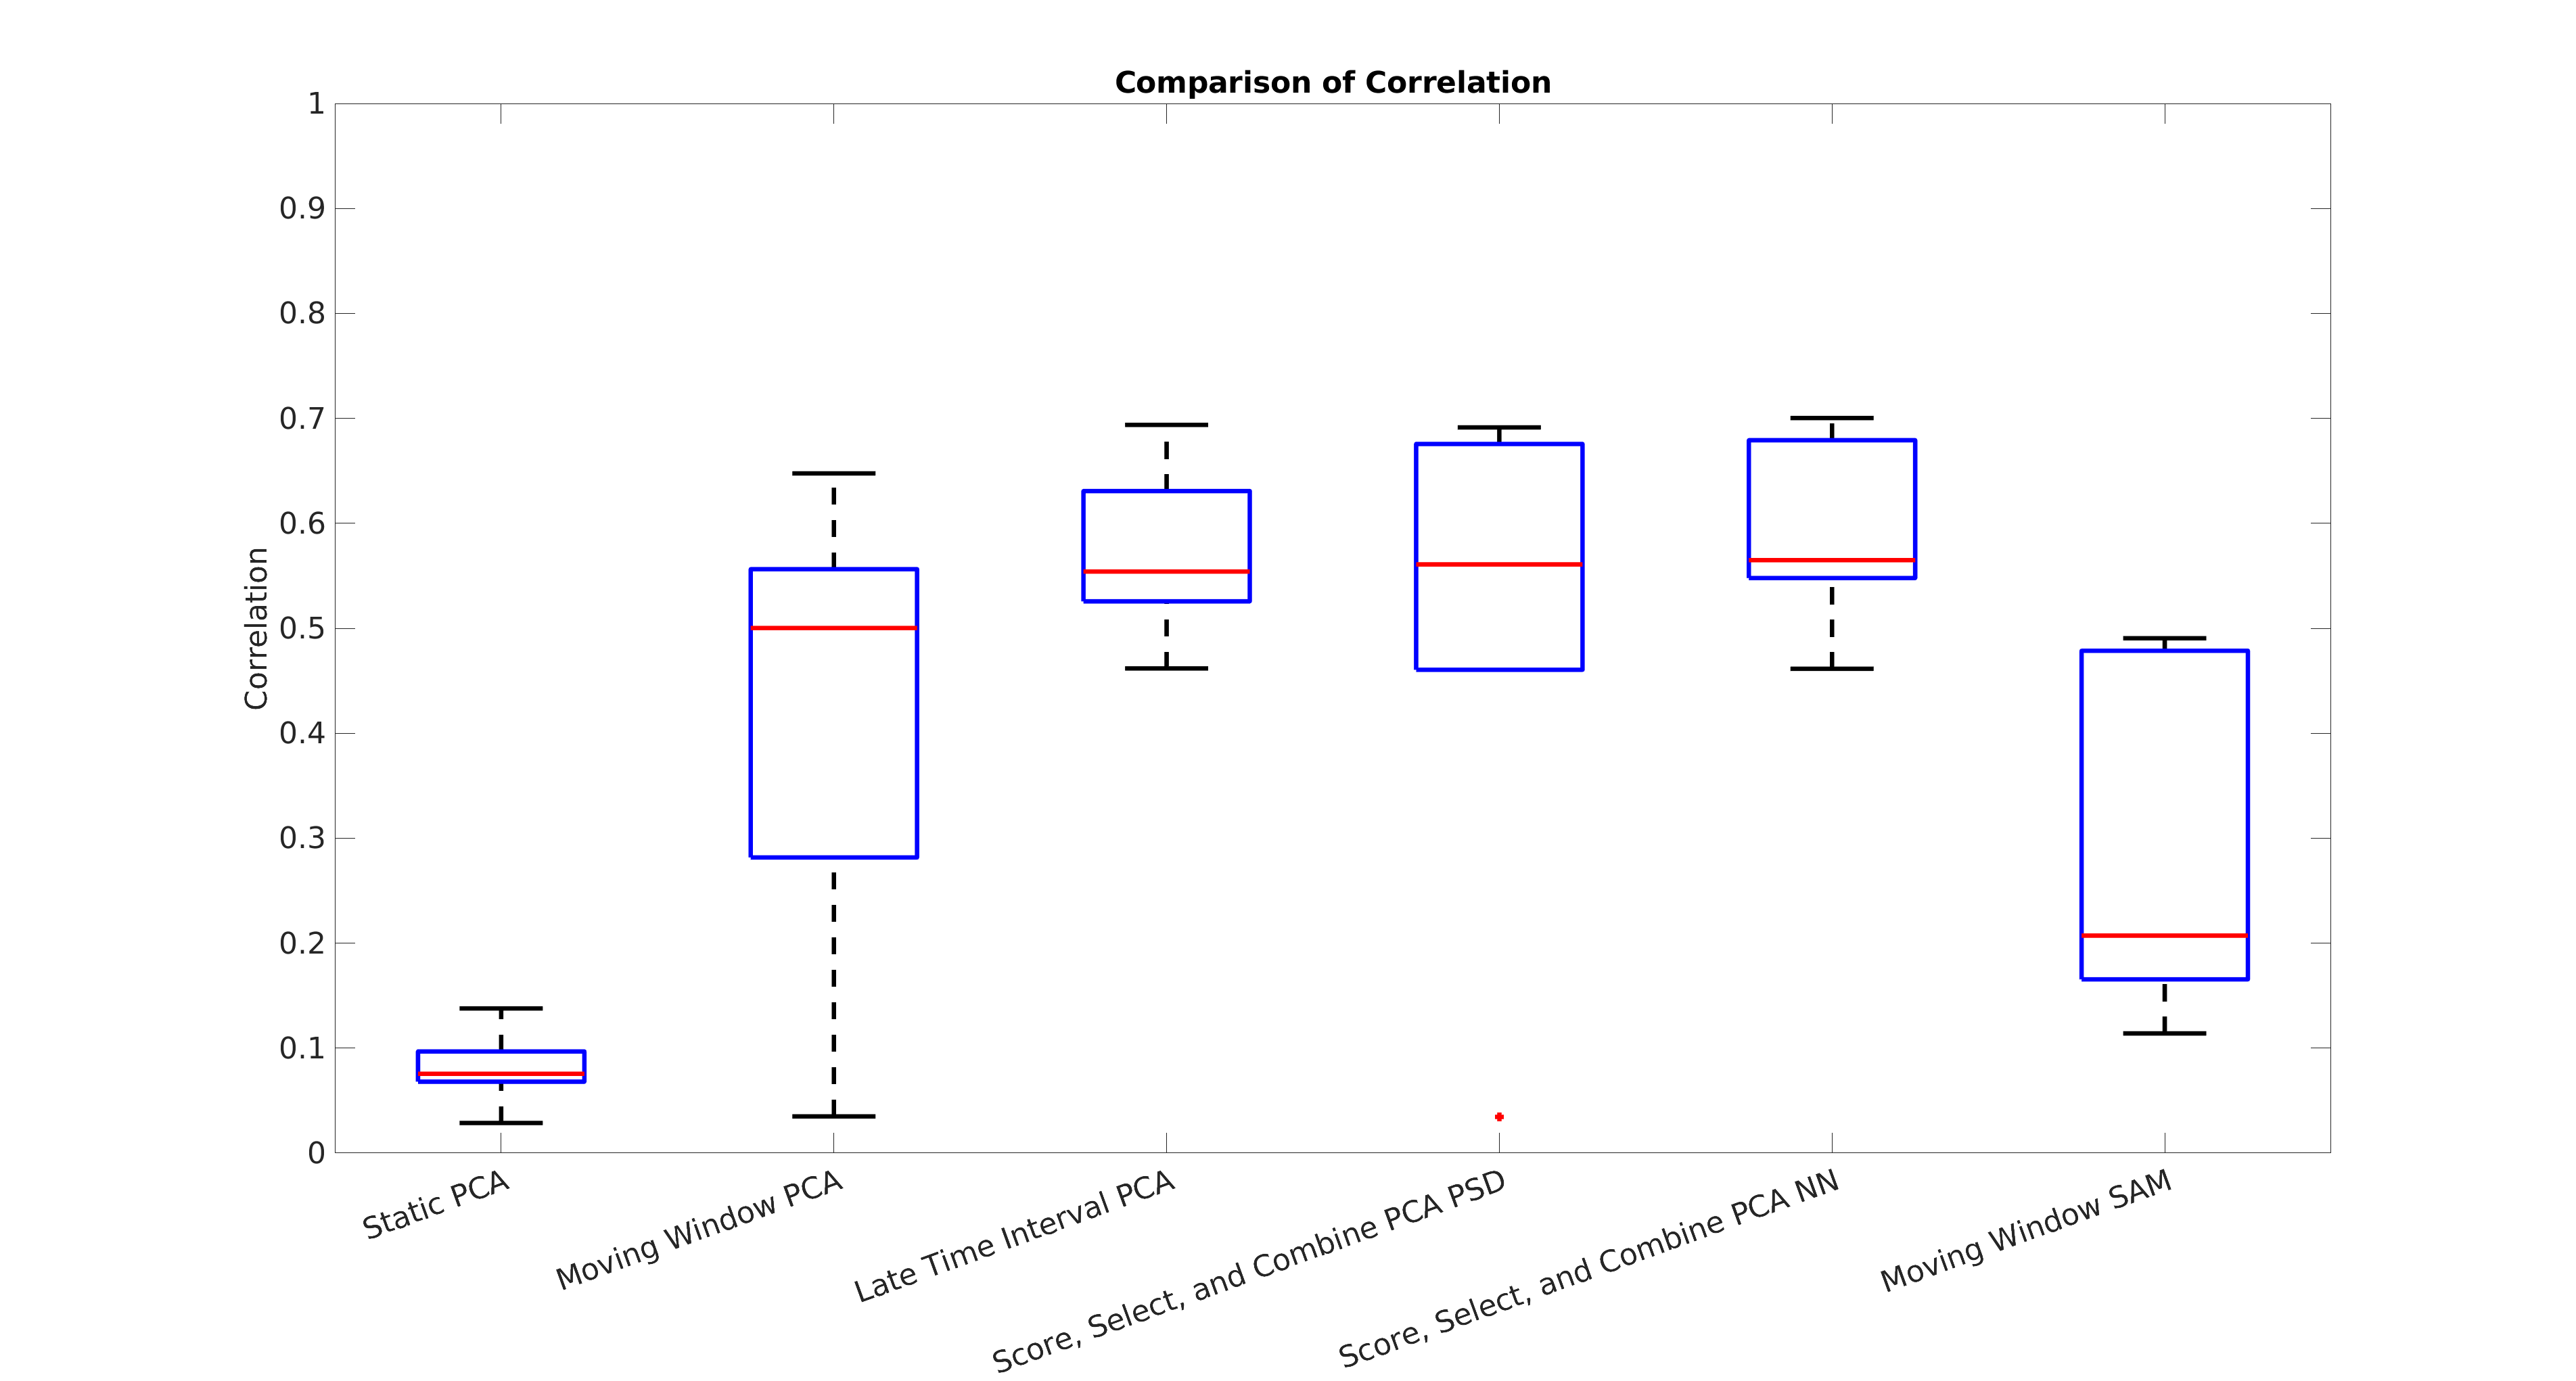
\includegraphics[width=1.0\linewidth]{figures/data_driven_surrogate_signal_extraction_methods_1_box_plot_all.png}
                
                \captionsetup{singlelinecheck=false}
                \caption{
                    A box plot showing for each method its correlation coefficient to the \gls{RPM} for the entire acquisition (taken for seven acquisitions). This is for Conventional \gls{PCA}, Moving Window \gls{PCA}, Late Time Interval \gls{PC}, Score, Select, and Combine using frequency and \gls{NN} scoring, and the Moving Window \gls{SAM} method.
                }
                \label{fig:box_plot_all}
            \end{figure}
            
            \begin{figure}
                \centering
                
                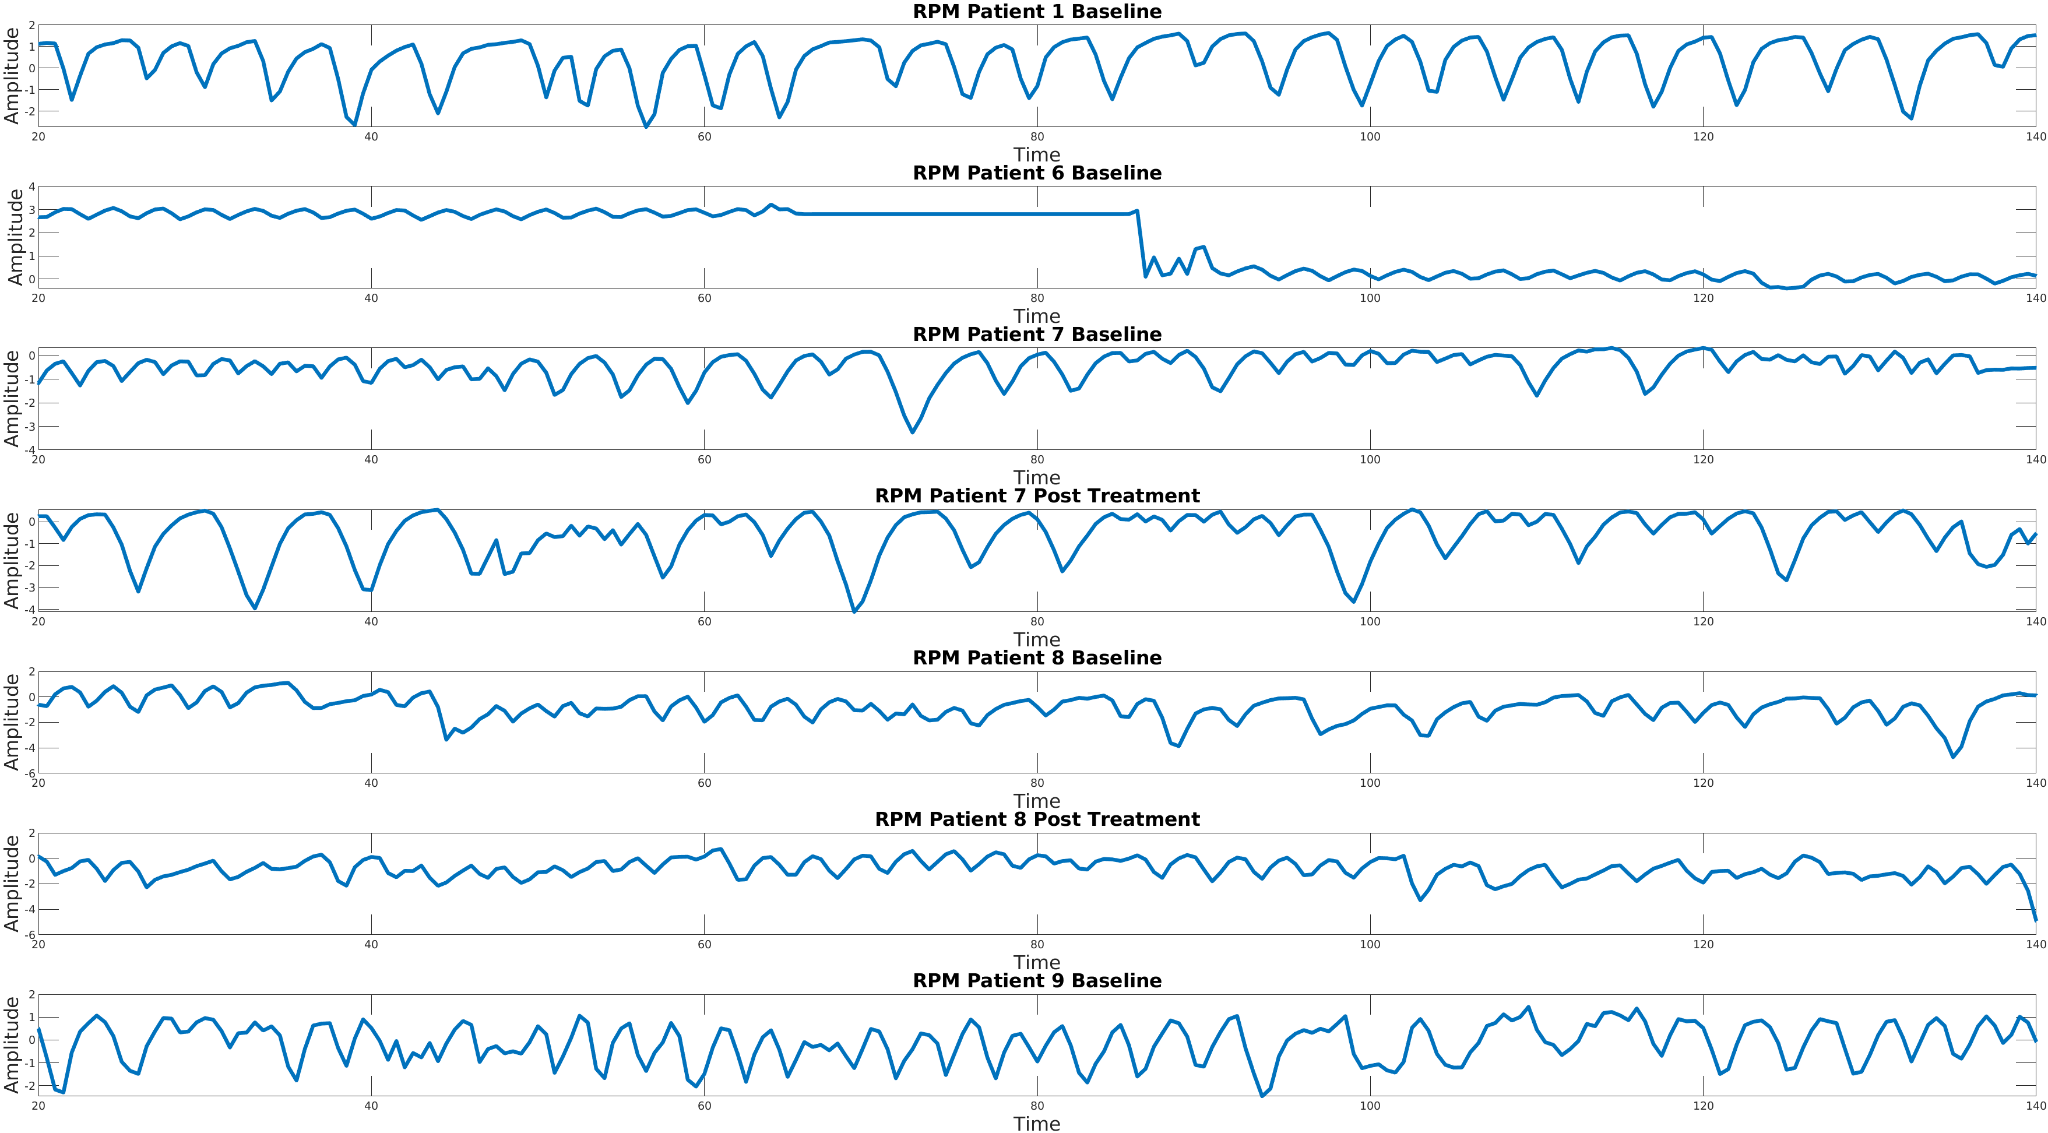
\includegraphics[width=1.0\linewidth]{figures/data_driven_surrogate_signal_extraction_methods_1_rpm_signals.png}
                
                \captionsetup{singlelinecheck=false}
                \caption{
                    \gls{RPM} signals for the first usable \SI{120}{\second} (between \SI{20}{\second} and \SI{140}{\second}) (for seven acquisitions). Notice that only the first acquisition of patient one shows a steady trace with an average frequency, every other trace shows variable breathing or artefacts.
                }
                \label{fig:rpm_signals}
            \end{figure}
            
            \begin{figure}
                \centering
                
                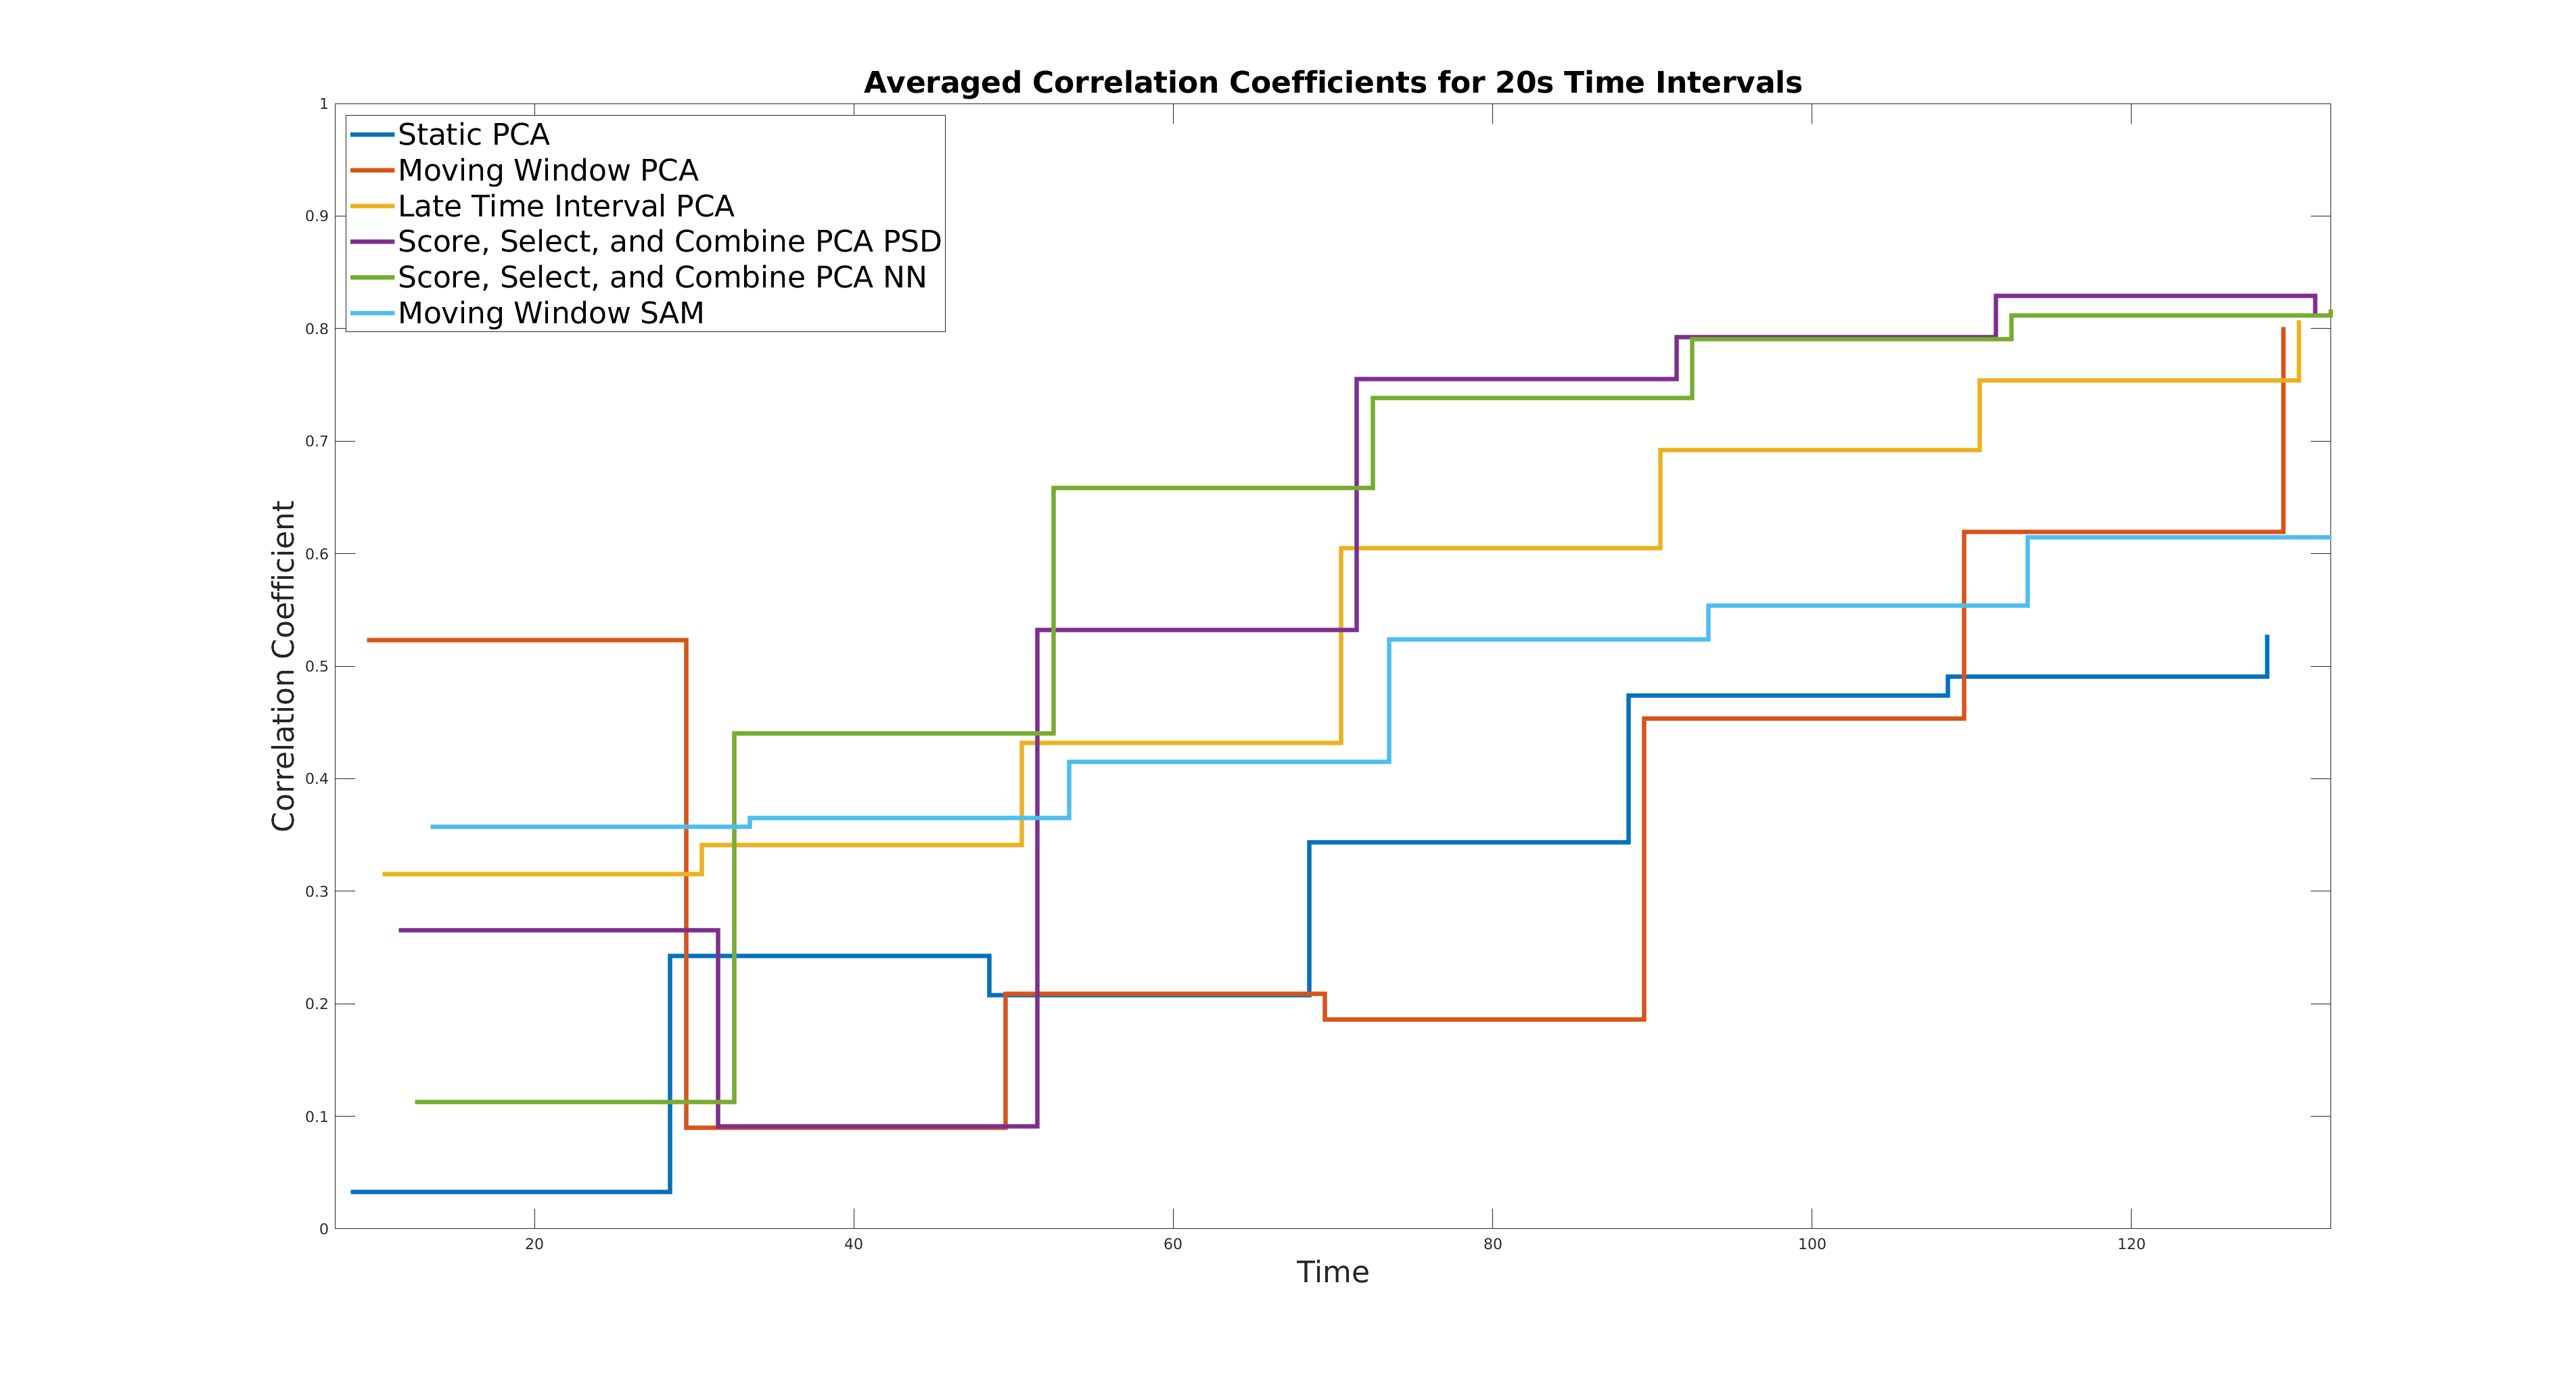
\includegraphics[width=1.0\linewidth]{figures/data_driven_surrogate_signal_extraction_methods_1_all_correlation_coefficient.png}
                
                \captionsetup{singlelinecheck=false}
                \caption{
                    Correlation coefficients to the \gls{RPM} for the first \SI{120}{\second} in \SI{20}{\second} intervals (between \SI{20}{\second} and \SI{140}{\second}) (taken as a mean for all data sets). This is for Conventional \gls{PCA}, Moving Window \gls{PCA}, Late Time Interval \gls{PC}, Score, Select, and Combine using frequency and \gls{NN} scoring, and the Moving Window \gls{SAM} method. The stair plots are staggered for the different methods for visual clarity.
                }
                \label{fig:all_cross_correlation}
            \end{figure}
            
            \begin{figure}
                \centering
                
                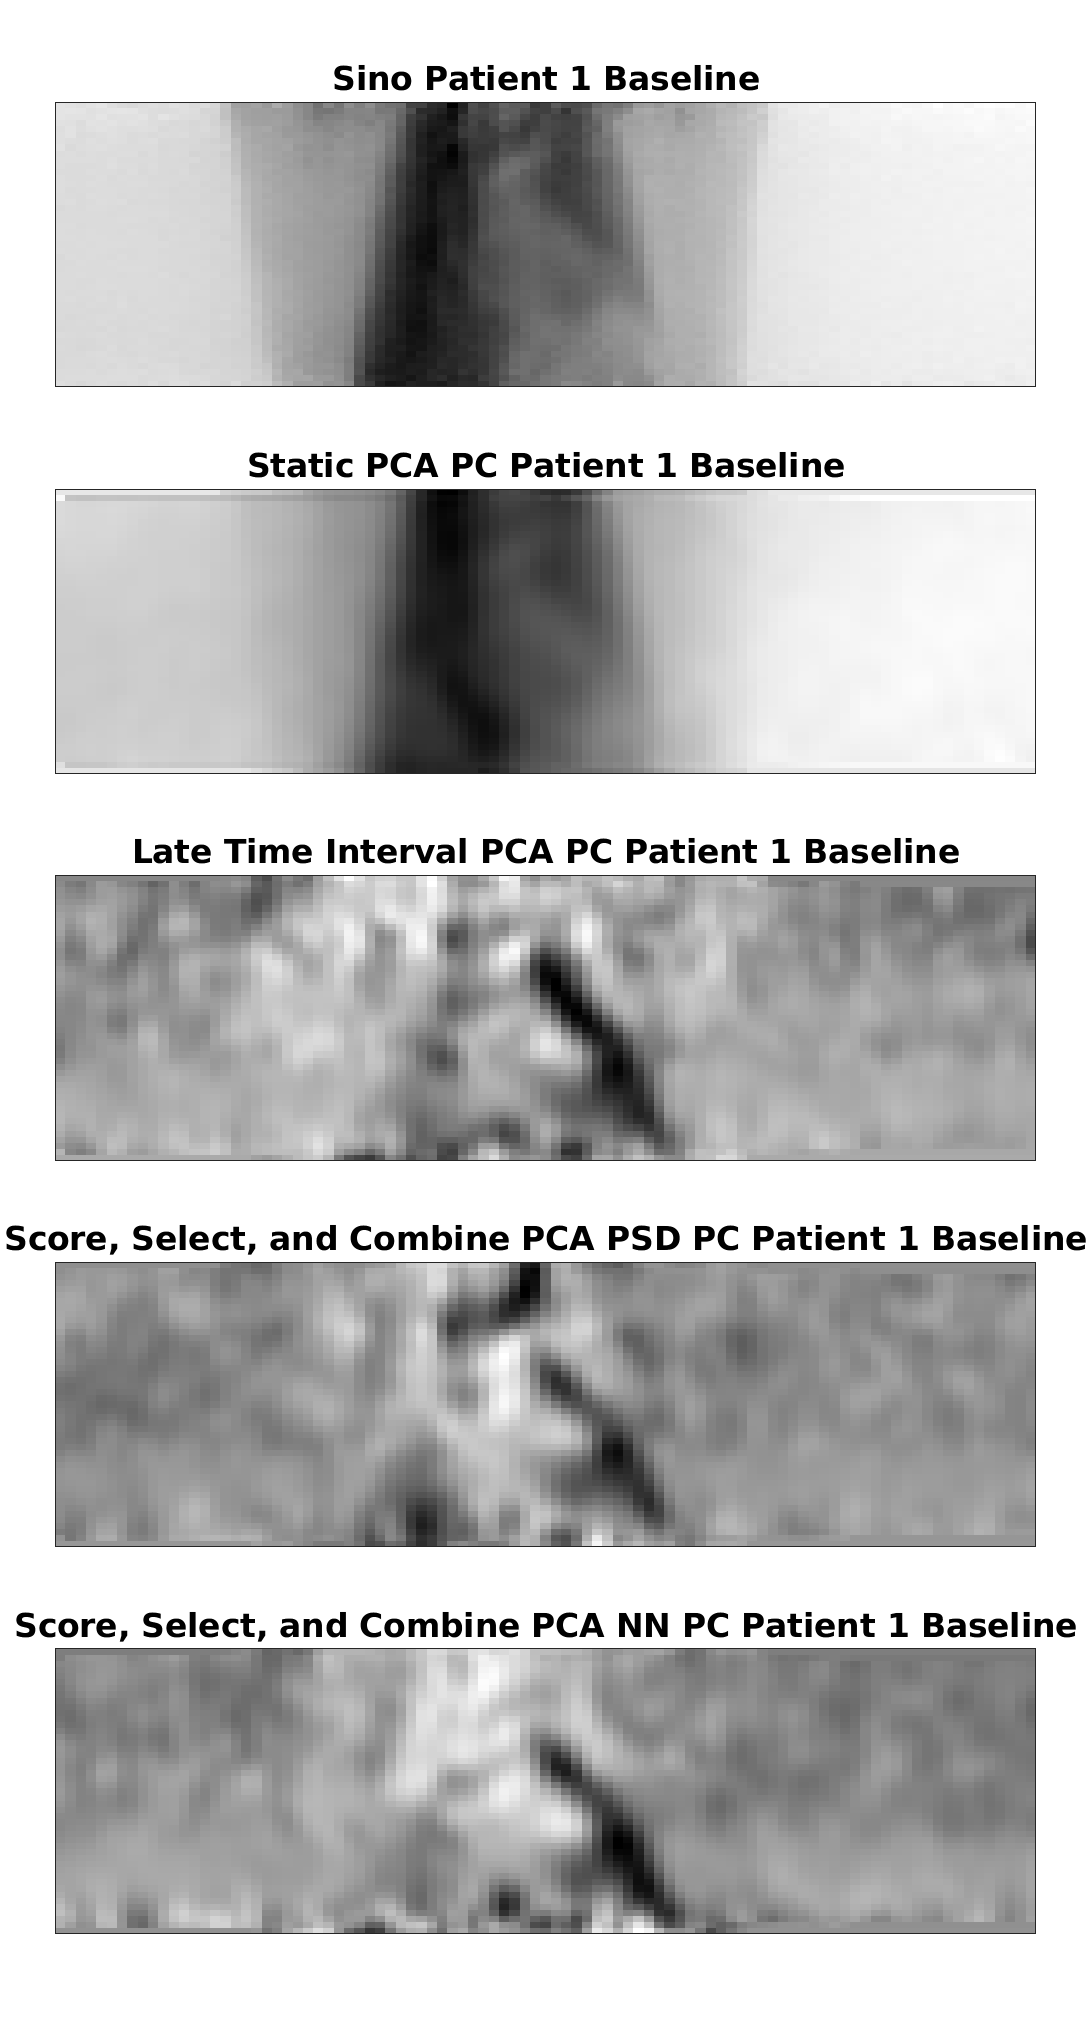
\includegraphics[width=0.7\linewidth]{figures/data_driven_surrogate_signal_extraction_methods_1_patient_one_pc_output.png}
                
                \captionsetup{singlelinecheck=false}
                \caption{
                    A plot showing a single `view' of the original PET data (top) as well as the \glspl{PC} used to generate the output signal for the Conventional, Late Time Interval and the two Score, Select, and Combine methods (taken for the first acquisition of patient eight).
                }
                \label{fig:patient_one_pc_output}
            \end{figure}
            
            A plot showing for each method its output compared to the \gls{RPM} for the first \SI{120}{\second} (between \SI{20}{\second} and \SI{140}{\second}) (taken for the first acquisition of patient one) can be seen in~\Fref{fig:patient_one_output}. From a visual analysis, it can be observed that the Conventional \gls{PCA} method has failed. Post normalisation it appears almost as if there is no variation in the signal at early time intervals. Both moving window methods show towards the end of the plot that they can extract a signal, however it takes until between \SI{60}{\second} and \SI{80}{\second} for both methods to begin to pick up the signal. For the \gls{SAM} based method it appears as if the sign determination method has failed before \SI{80}{\second}, regardless though the method still cannot extract a signal before \SI{60}{\second}. The Late Time Interval \gls{PC}, Score, Select, and Combine using frequency and \gls{NN} scoring methods all appear to be able to extract a usable signal right down to \SI{20}{\second} (around when counts begin to appear in the \gls{FOV}). The magnitude of the signal post \SI{80}{\second} more closely matches the \gls{RPM} (or in comparison to before \SI{80}{\second}) for both Select and Combine methods than for the Late Time Interval \gls{PC} method.
            
            A plot showing for each method its output compared to the \gls{RPM} for the first \SI{120}{\second} (between \SI{20}{\second} and \SI{140}{\second}) (taken for the first acquisition of patient eight) can be seen in~\Fref{fig:patient_eight_output}. Similar results as for in~\Fref{fig:patient_one_output} are repeated in~\Fref{fig:patient_eight_output}, although all methods match the \gls{RPM} worse than in~\Fref{fig:patient_one_output}. This acquisition was selected to be shown due to it being a difficult trace to extract. Regardless, the Late Time Interval \gls{PC} and Select and Combine methods appear to have extracted a signal early into the acquisition (from about \SI{35}{\second} on this patient).
            
            A box plot showing for each method its correlation coefficient to the \gls{RPM} for both the first \SI{120}{\second} (between \SI{20}{\second} and \SI{140}{\second}) and also for the entire acquisition (taken for seven acquisitions) can be seen in~\Fref{fig:box_plot_early} and~\Fref{fig:box_plot_all}. The correlation coefficient for the Conventional \gls{PCA} method is as would be expected, the correlation coefficient is low and as such the method is not usable. The correlation coefficients for both the moving window methods are roughly around $0.5$, indicating  that the Moving Window method is beneficial regardless of the method used to extract the signal for each window. However, again here the correlation coefficient is lower than is acceptable. The results from the Late Time Interval \gls{PC}, Score, Select, and Combine using frequency and \gls{NN} scoring methods all show correlation coefficients around $0.6$ or higher for both the early time interval as well as for all data. The Score, Select, and Combine methods show marginally higher correlation coefficient than the Late Time Interval \gls{PC} method and the \gls{NN} shows slightly higher correlation coefficient than the frequency based scoring.
            
            A plot showing for each method the evolution of the correlation coefficient with the \gls{RPM} over time for the first \SI{120}{\second} by computing it in \SI{20}{\second} intervals can be seen in~\Fref{fig:all_cross_correlation}. It can be observed that on average across all data sets all methods struggle to produce usable results at the very beginning of the acquisition (around when counts begin to appear in the \gls{FOV}). However, it is also apparent that on average both Score, Select, and Combine methods robustly begin to produce results which closely match the \gls{RPM}, as evidenced by a reasonable correlation past the first \SI{40}{\second} on most acquisitions. The Moving Window method appears to perform well in the first interval. However, correlation from the first interval is potentially misleading due to a discrepancy with when the tracer is injected and then when counts appear in the \gls{FOV}. In other words, results from the first interval should be considered with the context of the following intervals.
            
            A plot showing the component (or their combination) used to generate the output signal can be seen in~\Fref{fig:patient_one_pc_output}.
        
            One advantage of the sinogram-based methods is that the \gls{PC} (or signed mask for \gls{SAM}) can be visualised to see how it corresponds to anatomy and tracer uptake. In~\Fref{fig:patient_one_pc_output} it can be seen that the Conventional \gls{PCA} method returns a \gls{PC} which closely resembles the input data, leading to the conclusion that the variation in the selected \gls{PC} is dominated by the kinetics. The other methods produce a \gls{PC} which is more related to edges of internal structures where respiratory movement occurs. A visual inspection indicates that the least confounding variation and noise is included in the Score, Select, and Combine method using the \gls{NN} scoring method. Curiously it appears that the Late Time Interval and the Score, Select, and Combine method using the \gls{NN} scoring method return very similar distributions. However, the Score, Select, and Combine method using the frequency scoring method also returns a high value region in tissue at the top of the image.

            Plots showing a comparison of results achieved with and without pre- and post-processing can be seen in~\Fref{sec:pca_data_driven_surrogate_signal_extraction_methods_for_dynamic_pet_results_with_and_without_pre_and_post_processing_appendix}.

        \subsection{Discussion} \label{sec:pca_data_driven_surrogate_signal_extraction_methods_for_dynamic_pet_discussion}
            This section introduces several methods for \gls{DD} extraction of a respiratory signal from dynamic \gls{PET} data. From an examination of the literature, this appears to have only potentially been attempted in~\parencite{Schleyer2014}. Data used here are from a \gls{18F-FDG} study on patients with \gls{IPF}, while in the latter paper, \gls{13N-NH3} data was used to evaluate the proposed \gls{KRG} method.
            
            The work presented here suffers from a few limitations. Firstly, the data used here all originates from the same study, using the same procedure, the same radiotracer, and acquired on the same scanner. In order to better validate the generalisability of the method it would be positive to test on data acquired on different scanners and using different radiotracers. Additionally, from the data acquired only a subset of this data is usable due to issues during acquisition, the number of participants is limited. It would be beneficial to test the methods on a larger sample of patients, with both a larger number of non-complex and complex breathers to better test the limitations of the methods.
            
            An additional concern is the point at which the methods may fail for patients who exhibit abnormal breathing patterns. For instance, extremely slow breathers will breathe at a rate less than \SI{0.1}{\hertz}, which here would be considered to be radiotracer kinetics in the Score, Select, and Combine method using the frequency scoring method. Furthermore, this method also struggles with patients who breathe less regularly. The discrepancy between the results for the \gls{SAM} Moving Window method, presented here, and the \gls{KRG} ones shown in~\parencite{Schleyer2014} could also be attributed to this complexity. Many of the patients breathed at varying rates, stopped breathing during acquisition, or breathed unusually fast or slow (this is shown in~\Fref{fig:rpm_signals}). This was probably due to the data being acquired for an \gls{IPF} study.
        
            A limitation of the concept of using \glspl{SS} at all in the pursuit of the motion correction of respiratory motion is that a transform from the \gls{1D} \gls{SS} to the \gls{3D} motion is possible. There are methods, such as one using a \gls{MM} parameterised by the \gls{SS}~\parencite{McClelland2017, McClelland2013}. However, they are not trivial, and in the case where a \gls{1D} \gls{SS} is used, limit breath to breath variability and hysteresis to being periodic~\parencite{Whitehead2021ComparisonMap}.
        
            In the future, research will focus on further development of the method, including optimisation of the \gls{NN} scoring method. In the next stage, these methods will be applied to the task of implementing advanced respiratory motion correction on dynamic \gls{PET} data.

        \subsection{Conclusion} \label{sec:pca_data_driven_surrogate_signal_extraction_methods_for_dynamic_pet_conclusion}
            Several methods for extraction of a respiratory signal from dynamic \gls{PET} data have been presented and evaluated. Results from a visual comparison of early time interval output signals compared to the \gls{RPM}, quality of \gls{PC} and correlation coefficient of the output signals to the \gls{RPM} indicates that the Late Time Interval \gls{PC} and both Score, Select, and Combine methods are more robust and afford higher quality signals than moving window methods. The results also indicate that both Score, Select, and Combine methods can give a higher correlation coefficient earlier than the Late Time Interval \gls{PC} method and that scoring using the \gls{NN} shows slightly higher correlation coefficients than the frequency based scoring.
        
            In the future, research will focus on further development of the method, including optimisation of the \gls{NN} scoring method. In the next stage, these methods will be applied to the task of implementing advanced respiratory motion correction on dynamic \gls{PET} data.
    
%    \section{Feasibility Study of Neural Network Based Data Driven Surrogate Signal Extraction Methods for Dynamic PET} \label{sec:feasibility_study_of_neural_network_based_data_driven_surrogate_signal_extraction_methods_for_dynamic_pet}
        
        
%        \subsection{Introduction} \label{sec:feasibility_study_of_neural_network_based_data_driven_surrogate_signal_extraction_methods_for_dynamic_pet_introduction}
            
        
%        \subsection{Methods} \label{sec:feasibility_study_of_neural_network_based_data_driven_surrogate_signal_extraction_methods_for_dynamic_pet_methods}
            
            
%        \subsection{Results} \label{sec:feasibility_study_of_neural_network_based_data_driven_surrogate_signal_extraction_methods_for_dynamic_pet_results}
            
            
%        \subsection{Discussion and Conclusion} \label{sec:feasibility_study_of_neural_network_based_data_driven_surrogate_signal_extraction_methods_for_dynamic_pet_discussion_and_conclusion}
